\section{Thực nghiệm và phân tích kết quả}
\label{sec:experiments}

Chương này đánh giá hai mô hình đề xuất trên bộ dữ liệu Amazon Electronics. Mục~\ref{sec:data} mô tả dữ liệu và tiền xử lý, Mục~\ref{sec:protocol} trình bày giao thức đánh giá. Hai mục kết quả được tách theo nhóm: Mục~\ref{sec:grnr-results} so GRNR với các mô hình giải trực tiếp, Mục~\ref{sec:dfhf-results} so DFHF với các mô hình cần huấn luyện. Mục~\ref{sec:demo} giới thiệu hệ thống demo và Mục~\ref{sec:discussion} thảo luận các giới hạn. Mọi kết quả đều đo trên tập validation, với một seed (42).

\subsection{Dữ liệu và tiền xử lý}
\label{sec:data}

\subsubsection{Nguồn dữ liệu}

Dữ liệu là danh mục Electronics của bộ Amazon product data do McAuley và cộng sự công bố~\cite{mcauley2015image,he2016ups}. Dự án dùng tệp đánh giá bản 5-core (mỗi người dùng và sản phẩm có ít nhất 5 đánh giá) và tệp metadata của danh mục này từ trang SNAP. Từ tệp đánh giá, dự án lấy mã người đánh giá (\texttt{reviewerID}), mã sản phẩm (\texttt{asin}), số sao (\texttt{overall}) và thời điểm (\texttt{unixReviewTime}); từ tệp metadata, dự án lấy tên, thương hiệu và danh mục sản phẩm. Đây là các đánh giá công khai, không phải nhật ký mua hàng; một đánh giá từ 4 sao trở lên chỉ được xem là tín hiệu gián tiếp cho sở thích.

\subsubsection{Quy trình tiền xử lý}

\figref{fig:pipeline} tóm tắt các bước biến dữ liệu thô thành các tập dùng cho thực nghiệm; \tabref{tab:filter} ghi số tương tác còn lại sau mỗi bước, lấy từ sổ ghi nhận quá trình lọc của bộ dữ liệu.

\begin{figure}[htbp]
\centering
\begin{tikzpicture}[node distance=0.55cm and 0.5cm, every node/.style={font=\small}]
\node[chthreeblue, text width=3.1cm] (raw) {Đánh giá thô\\1.689.188};
\node[chthreeblue, text width=3.1cm, right=of raw] (pos) {Giữ rating $\ge4$\\1.356.067};
\node[chthreeblue, text width=3.1cm, right=of pos] (core) {K-core $\ge5$ (13 vòng)\\1.072.740};
\node[chthreegreen, text width=3.1cm, below=of core] (split) {Chia theo thời gian\\80/10/10};
\node[chthreepurple, text width=3.1cm, left=of split] (sparse) {Giảm train\\$d\in\{1;\,0{,}75;\,0{,}5;\,0{,}25\}$};
\node[chthreeorange, text width=3.1cm, left=of sparse] (models) {Huấn luyện và đánh giá trên validation};
\draw[chthreeflow] (raw) -- (pos);
\draw[chthreeflow] (pos) -- (core);
\draw[chthreeflow] (core) -- (split);
\draw[chthreeflow] (split) -- (sparse);
\draw[chthreeflow] (sparse) -- (models);
\end{tikzpicture}
\caption[Quy trình tiền xử lý dữ liệu]{Quy trình tiền xử lý dữ liệu. Số trong mỗi ô là số tương tác còn lại sau bước đó.}
\label{fig:pipeline}
\end{figure}

\begin{table}[htbp]
\centering
\caption[Số tương tác qua từng bước tiền xử lý]{Số tương tác qua từng bước tiền xử lý.}
\label{tab:filter}
\begin{tabular}{@{}lrr@{}}
\toprule
Bước & Còn lại & Bị loại \\
\midrule
Đánh giá thô & 1.689.188 & --- \\
Giữ đánh giá có rating $\ge 4$ & 1.356.067 & 333.121 \\
Khử trùng cặp (người dùng, sản phẩm) & 1.356.067 & 0 \\
K-core hai phía ($\ge5$ cho người dùng và sản phẩm) & 1.072.740 & 283.327 \\
\bottomrule
\end{tabular}
\end{table}

Đầu tiên, các đánh giá có rating từ 4 trở lên được giữ làm phản hồi tích cực. Sau đó các cặp (người dùng, sản phẩm) trùng lặp được khử, giữ bản mới nhất và rating cao nhất; trên dữ liệu này không có cặp trùng. Dù tệp nguồn đã là 5-core, việc bỏ các đánh giá thấp làm nhiều người dùng và sản phẩm rơi xuống dưới 5 tương tác, nên bộ lọc K-core hai phía được áp lại cho đến khi hội tụ. Vòng đầu loại 213.614 tương tác, các vòng sau giảm dần, và quá trình dừng sau 13 vòng. Cuối cùng, người dùng và sản phẩm được đánh lại chỉ số liên tục theo thứ tự mã gốc, nên kết quả tái lập được.

\begin{table}[htbp]
\centering
\caption[Thống kê dữ liệu sau tiền xử lý]{Thống kê dữ liệu sau tiền xử lý. Tính trên toàn bộ tương tác, trước khi chia tập.}
\label{tab:data-stats}
\begin{tabular}{@{}lr@{}}
\toprule
Thống kê & Giá trị \\
\midrule
Số người dùng & 124.895 \\
Số sản phẩm & 44.843 \\
Số tương tác & 1.072.740 \\
Mật độ & 0,0192\% \\
Số tương tác mỗi người dùng: trung bình / trung vị / lớn nhất & 8,59 / 6 / 354 \\
Số tương tác trung bình mỗi sản phẩm & 23,9 \\
\bottomrule
\end{tabular}
\end{table}

\subsubsection{Chia tập theo thời gian}

Lịch sử của mỗi người dùng được sắp theo thời điểm đánh giá; các tương tác cùng thời điểm được sắp theo một hàm băm có seed của cặp (người dùng, sản phẩm), rồi theo mã sản phẩm. Sau đó 107.274 người dùng được chọn ngẫu nhiên (seed 42) trong số người dùng có ít nhất 3 tương tác; sau K-core, mọi người dùng đều thỏa điều kiện này. Với mỗi người dùng được chọn, tương tác cuối cùng đưa vào test, tương tác áp cuối đưa vào validation, phần còn lại vào train. 17.621 người dùng còn lại chỉ có trong train. Tỉ lệ 80/10/10 vì vậy được tính trên \emph{tổng số tương tác}, không phải trên từng người dùng, và không có một mốc thời gian chung cho cả tập dữ liệu (\tabref{tab:split}).

\begin{table}[htbp]
\centering
\caption[Kết quả chia tập theo thời gian]{Kết quả chia tập theo thời gian.}
\label{tab:split}
\begin{tabular}{@{}lrrr@{}}
\toprule
 & Train & Validation & Test \\
\midrule
Số tương tác & 858.192 & 107.274 & 107.274 \\
Tỉ lệ & 80\% & 10\% & 10\% \\
Mục tiêu có sản phẩm không xuất hiện trong train & --- & 59 & 187 \\
\bottomrule
\end{tabular}
\end{table}

Kiểm tra sau khi chia không tìm thấy cặp (người dùng, sản phẩm) nào xuất hiện ở hai tập, và không có vi phạm thứ tự thời gian. Tuy nhiên, toàn bộ thời điểm trong dữ liệu đều nằm đúng nửa đêm, tức chỉ chính xác đến ngày. Do đó có 45.431 người dùng có tương tác validation cùng ngày với tương tác train cuối cùng, và 42.592 người dùng có tương tác test cùng ngày với tương tác validation. Thứ tự thời gian vì thế chỉ là ``không giảm''; giao thức này không bảo đảm mô phỏng việc dự đoán tương lai một cách nghiêm ngặt~\cite{ji2023leakage}. Để giữ thứ tự thời gian, dự án không chuyển tương tác của sản phẩm chưa xuất hiện sang train. 40 sản phẩm không có trong train; 59 mục tiêu validation thuộc các sản phẩm này bị loại khỏi phép đo.

\subsubsection{Tạo các mức giảm tương tác}
\label{sec:sparsity-protocol}

Để khảo sát ảnh hưởng của độ thưa, tập train được giảm xuống bốn tỉ lệ $d=1$; $0{,}75$; $0{,}5$ và $0{,}25$; validation và test giữ nguyên. Thuật toán giảm (seed 42) gán cho mỗi cạnh một số ngẫu nhiên, rồi xây dựng một \emph{lõi phủ}: cạnh đầu tiên (theo thứ tự ngẫu nhiên) của mỗi sản phẩm, sau đó cạnh đầu tiên của mỗi người dùng chưa được phủ. Các cạnh còn lại được thêm theo thứ tự ngẫu nhiên cho đến khi đủ $\mathrm{round}(d\cdot|E|)$ cạnh. Nhờ lõi phủ, mọi người dùng và sản phẩm vẫn còn ít nhất một tương tác ở mọi mức $d$.

\begin{table}[htbp]
\centering
\caption[Tập huấn luyện ở các mức giảm tương tác]{Tập huấn luyện ở các mức giảm tương tác. Người dùng bậc 1 là người dùng có sản phẩm mục tiêu trong tập ứng viên nhưng chỉ còn đúng một tương tác huấn luyện.}
\label{tab:sparsity}
\begin{tabular}{@{}lrrrr@{}}
\toprule
$d$ & 1 & 0,75 & 0,5 & 0,25 \\
\midrule
Số cạnh & 858.192 & 643.644 & 429.096 & 214.548 \\
Số cạnh trung bình mỗi người dùng & 6,87 & 5,15 & 3,44 & 1,72 \\
Người dùng warm bậc 1 & 0 & 6.657 & 28.555 & 72.944 \\
Tỉ lệ người dùng warm bậc 1 & 0\% & 6,2\% & 26,6\% & 68,0\% \\
\bottomrule
\end{tabular}
\end{table}

Ở mọi mức, số cạnh đúng bằng số yêu cầu (\tabref{tab:sparsity}). Cần lưu ý hai hệ quả. Thứ nhất, việc giảm \emph{không ngẫu nhiên đều}: người dùng ít tương tác được lõi phủ bảo vệ, nên người dùng nhiều tương tác mất tỉ lệ lớn hơn. Thứ hai, ở $d=0{,}25$ có tới 68\% người dùng warm chỉ còn một tương tác. Ở mức này, bài toán gần với việc gợi ý từ một sản phẩm duy nhất, và một xếp hạng theo độ phổ biến trở nên rất cạnh tranh (Mục~\ref{sec:discussion}). Mỗi mức $d$ chỉ được lấy mẫu một lần và dùng chung cho mọi mô hình.

\subsubsection{Vai trò của từng phần dữ liệu}

\tabref{tab:data-roles} tổng kết phần dữ liệu nào được dùng ở đâu. Tập test không được dùng trong báo cáo. Kiểm kê các tệp kết quả không tìm thấy điểm test nào được lưu, nhưng kiểm kê này không chứng minh được rằng tập test chưa từng được xem.

\begin{table}[htbp]
\centering
\caption[Vai trò của từng phần dữ liệu]{Vai trò của từng phần dữ liệu.}
\label{tab:data-roles}
\begin{tabularx}{\textwidth}{@{}lX@{}}
\toprule
Phần dữ liệu & Vai trò \\
\midrule
Train giữ lại theo $d$ & Đầu vào huấn luyện của mọi mô hình; xác định tập ứng viên \\
Train gốc ($d=1$) & Loại các sản phẩm đã tương tác khỏi danh sách gợi ý ở mọi $d$; định nghĩa nhóm người dùng theo số tương tác \\
Validation & Chọn cấu hình và checkpoint, \emph{đồng thời} dùng để báo cáo kết quả \\
Test & Không dùng \\
Metadata sản phẩm & Chỉ hiển thị trong demo; không mô hình nào dùng để xếp hạng \\
\bottomrule
\end{tabularx}
\end{table}

Metadata có 888 sản phẩm thiếu tên (2,0\%) và 7.351 sản phẩm thiếu thương hiệu (16,4\%). Vì metadata không tham gia xếp hạng, các thiếu sót này chỉ ảnh hưởng đến phần hiển thị của demo. Pipeline còn tạo embedding văn bản và tập tương tác bị đánh giá thấp (rating dưới 4), nhưng không mô hình nào trong báo cáo sử dụng chúng.

\subsection{Thiết lập và giao thức đánh giá}
\label{sec:protocol}

\textbf{Mô hình và cấu hình.} \tabref{tab:setup} liệt kê các mô hình trong hai nhóm. DirectAU dùng encoder LightGCN theo cấu hình tham chiếu của tác giả. EASE có hai biến thể: EASE đầy đủ dùng toàn bộ ma trận trọng số $|\mathcal{I}|\times|\mathcal{I}|$, còn EASE top-128 chỉ giữ 128 trọng số lớn nhất mỗi cột để lưu trữ. Các baseline neural dùng embedding 64 chiều, 3 lớp, Adam với tốc độ học $3\cdot10^{-4}$, lô 2.048 và chạy đủ 200 epoch.

\begin{table}[htbp]
\centering
\caption[Cấu hình và môi trường chạy của các mô hình]{Cấu hình và môi trường chạy của các mô hình.}
\label{tab:setup}
\small
\begin{tabularx}{\textwidth}{@{}llXl@{}}
\toprule
Nhóm & Mô hình & Cấu hình chính & Phần cứng \\
\midrule
\multirow{4}{*}{Giải trực tiếp} & GRNR & \tabref{tab:grnr-hparams} & Cholesky CPU, 1 luồng \\
 & EASE đầy đủ~\cite{steck2019ease} & $\lambda=300$ & CPU \\
 & EASE top-128 & EASE đầy đủ, cắt 128 trọng số/cột & CPU \\
 & GF-CF~\cite{shen2021gfcf} & 256 vector kỳ dị, trọng số lọc lý tưởng 0,3 & CPU \\
\midrule
\multirow{4}{*}{Cần huấn luyện} & DFHF & \tabref{tab:dfhf-hparams} & GPU Tesla T4 \\
 & LightGCN~\cite{he2020lightgcn} & 64 chiều, 3 lớp, BPR & GPU Tesla T4 \\
 & XSimGCL~\cite{yu2023xsimgcl} & Trọng số tương phản 0,1; $\tau=0{,}2$; $\epsilon=0{,}1$ & GPU Tesla T4 \\
 & DirectAU~\cite{wang2022directau} & Encoder LightGCN; $\gamma=1$ & GPU Tesla T4 \\
\bottomrule
\end{tabularx}
\end{table}

\textbf{Cách xếp hạng.} Với mỗi người dùng, mô hình chấm điểm mọi sản phẩm trong tập ứng viên (44.803 sản phẩm ở $d=1$), loại các sản phẩm đã có trong train gốc, rồi lấy top-$K$. Dự án không dùng cách lấy mẫu một số sản phẩm âm để so, vì các thước đo tính trên mẫu có thể cho thứ tự mô hình khác với xếp hạng đầy đủ~\cite{krichene2020sampled}. Phép đo chỉ tính trên 107.215 người dùng warm; tập này giống nhau cho mọi mô hình ở mọi $d$.

\textbf{Thước đo.} Mỗi người dùng warm có đúng một sản phẩm mục tiêu trong validation. Với $r_u$ là vị trí của sản phẩm mục tiêu trong danh sách gợi ý,
\begin{equation}
\mathrm{Recall@}K = \frac{1}{|\mathcal{U}_w|}\sum_{u}\mathbb{1}[r_u\le K], \qquad
\mathrm{NDCG@}K = \frac{1}{|\mathcal{U}_w|}\sum_{u}\frac{\mathbb{1}[r_u\le K]}{\log_2(r_u+1)}.
\end{equation}
Báo cáo dùng $K=10$ và $K=20$, trong đó NDCG@20 là thước đo chính.

\textbf{Chọn cấu hình và checkpoint.} Trong nhóm cần huấn luyện, mọi mô hình đều chạy đủ 200 epoch và giữ checkpoint có NDCG@20 validation cao nhất. Cách chọn giống nhau trong nhóm, nhưng vì cùng tập validation vừa dùng để chọn vừa dùng để báo cáo, giá trị tuyệt đối của mọi mô hình trong nhóm đều bị nâng lên một cách lạc quan. Trong nhóm giải trực tiếp, cấu hình GRNR được chọn qua quá trình thử nghiệm của dự án, còn EASE và GF-CF dùng cấu hình cố định; ngân sách tinh chỉnh vì vậy không cân bằng~\cite{dacrema2019progress}.

\textbf{Kiểm định thống kê.} Với mỗi cặp (mô hình đề xuất, baseline cùng nhóm), lấy hiệu NDCG@20 của từng người dùng rồi bootstrap ghép cặp theo người dùng 10.000 lần để có khoảng tin cậy 95\% (phân vị) và giá trị $p$ một phía cho giả thuyết mô hình đề xuất tốt hơn. Ở mỗi mức $d$, mỗi nhóm có 3 so sánh; giá trị $p$ được hiệu chỉnh Holm trong nhóm 3 so sánh đó. Với 10.000 lần lặp, $p$ nhỏ nhất đo được là $(0+1)/(10^4+1)\approx10^{-4}$, nên báo cáo viết $p\le10^{-4}$. Khoảng tin cậy chưa được hiệu chỉnh đồng thời. Vì chỉ có một seed, khoảng tin cậy chỉ phản ánh biến động do tập người dùng, không phản ánh biến động giữa các lần huấn luyện.

\subsection{Graph-Regularized Neighborhood Regression so với các mô hình giải trực tiếp}
\label{sec:grnr-results}

\subsubsection{Chất lượng xếp hạng}

\tabref{tab:closed-form} cho kết quả của nhóm giải trực tiếp ở cả bốn mức $d$. Ở $d=1$, GRNR có NDCG@20 cao nhất nhóm (0,03829), tiếp theo là EASE đầy đủ (0,03796), EASE top-128 (0,03679) và GF-CF (0,01886). Theo \tabref{tab:closed-form-sig}, GRNR hơn EASE top-128 ($\Delta=+0{,}00150$, KTC 95\% $[0{,}00111;\,0{,}00189]$) và GF-CF ($\Delta=+0{,}01943$) với khoảng tin cậy không chứa 0. Tuy nhiên, chênh lệch với EASE đầy đủ rất nhỏ ($\Delta=+0{,}00033$, KTC $[-0{,}00007;\,0{,}00073]$, $p_{\mathrm{Holm}}=0{,}051$): chưa đủ bằng chứng để kết luận GRNR tốt hơn EASE đầy đủ theo phép so sánh này. Kết quả này cũng không chứng minh hai mô hình tương đương.

\begin{table}[htbp]
\centering
\caption[Chất lượng xếp hạng của các mô hình giải trực tiếp]{Chất lượng xếp hạng của các mô hình giải trực tiếp. Đo trên tập validation, seed 42; giá trị cao nhất ở mỗi mức $d$ được in đậm.}
\label{tab:closed-form}
\begin{tabular}{@{}llrrrr@{}}
\toprule
$d$ & Mô hình & NDCG@10 & NDCG@20 & Recall@10 & Recall@20 \\
\midrule
\multirow{4}{*}{1} & GRNR & \textbf{0,03292} & \textbf{0,03829} & \textbf{0,05629} & \textbf{0,07757} \\
 & EASE đầy đủ & 0,03287 & 0,03796 & 0,05607 & 0,07629 \\
 & EASE top-128 & 0,03206 & 0,03679 & 0,05413 & 0,07290 \\
 & GF-CF & 0,01573 & 0,01886 & 0,02788 & 0,04035 \\
\midrule
\multirow{4}{*}{0,75} & GRNR & \textbf{0,02545} & 0,02928 & \textbf{0,04319} & 0,05836 \\
 & EASE đầy đủ & \textbf{0,02545} & \textbf{0,02939} & 0,04303 & \textbf{0,05867} \\
 & EASE top-128 & 0,02448 & 0,02772 & 0,04068 & 0,05345 \\
 & GF-CF & 0,00668 & 0,00839 & 0,01237 & 0,01916 \\
\midrule
\multirow{4}{*}{0,5} & GRNR & 0,01465 & 0,01715 & 0,02417 & 0,03410 \\
 & EASE đầy đủ & \textbf{0,01658} & \textbf{0,01917} & \textbf{0,02710} & \textbf{0,03736} \\
 & EASE top-128 & 0,01564 & 0,01766 & 0,02496 & 0,03294 \\
 & GF-CF & 0,00268 & 0,00384 & 0,00547 & 0,01009 \\
\midrule
\multirow{4}{*}{0,25} & GRNR & \textbf{0,00573} & \textbf{0,00798} & \textbf{0,01113} & \textbf{0,02017} \\
 & EASE đầy đủ & 0,00534 & 0,00674 & 0,00956 & 0,01513 \\
 & EASE top-128 & 0,00438 & 0,00497 & 0,00703 & 0,00936 \\
 & GF-CF & 0,00205 & 0,00385 & 0,00511 & 0,01235 \\
\bottomrule
\end{tabular}
\end{table}

\begin{table}[htbp]
\centering
\caption[Kiểm định chênh lệch NDCG@20 trong nhóm giải trực tiếp]{Kiểm định chênh lệch NDCG@20 trong nhóm giải trực tiếp. Hiệu của GRNR trừ từng baseline; bootstrap ghép cặp theo người dùng 10.000 lần ($n=107.215$); giá trị $p$ một phía, hiệu chỉnh Holm trong mỗi mức $d$.}
\label{tab:closed-form-sig}
\begin{tabular}{@{}llrrr@{}}
\toprule
$d$ & So sánh & $\Delta$ NDCG@20 & KTC 95\% & $p_{\mathrm{Holm}}$ (một phía) \\
\midrule
\multirow{3}{*}{1} & GRNR $-$ EASE đầy đủ & $+0{,}00033$ & $[-0{,}00007;\;+0{,}00073]$ & 0,051 \\
 & GRNR $-$ EASE top-128 & $+0{,}00150$ & $[+0{,}00111;\;+0{,}00189]$ & $\le 3\cdot10^{-4}$ \\
 & GRNR $-$ GF-CF & $+0{,}01943$ & $[+0{,}01874;\;+0{,}02010]$ & $\le 3\cdot10^{-4}$ \\
\midrule
\multirow{3}{*}{0,75} & GRNR $-$ EASE đầy đủ & $-0{,}00011$ & $[-0{,}00049;\;+0{,}00028]$ & 0,721 \\
 & GRNR $-$ EASE top-128 & $+0{,}00157$ & $[+0{,}00121;\;+0{,}00193]$ & $\le 3\cdot10^{-4}$ \\
 & GRNR $-$ GF-CF & $+0{,}02089$ & $[+0{,}02023;\;+0{,}02159]$ & $\le 3\cdot10^{-4}$ \\
\midrule
\multirow{3}{*}{0,5} & GRNR $-$ EASE đầy đủ & $-0{,}00202$ & $[-0{,}00237;\;-0{,}00167]$ & 1,000 \\
 & GRNR $-$ EASE top-128 & $-0{,}00051$ & $[-0{,}00082;\;-0{,}00021]$ & 1,000 \\
 & GRNR $-$ GF-CF & $+0{,}01331$ & $[+0{,}01276;\;+0{,}01386]$ & $\le 3\cdot10^{-4}$ \\
\midrule
\multirow{3}{*}{0,25} & GRNR $-$ EASE đầy đủ & $+0{,}00124$ & $[+0{,}00095;\;+0{,}00154]$ & $\le 3\cdot10^{-4}$ \\
 & GRNR $-$ EASE top-128 & $+0{,}00301$ & $[+0{,}00274;\;+0{,}00330]$ & $\le 3\cdot10^{-4}$ \\
 & GRNR $-$ GF-CF & $+0{,}00413$ & $[+0{,}00383;\;+0{,}00444]$ & $\le 3\cdot10^{-4}$ \\
\bottomrule
\end{tabular}
\end{table}

\subsubsection{Ảnh hưởng của mức độ thưa và nhóm người dùng}

\figref{fig:closed-density} và \tabref{tab:closed-form-sig} cho thấy so sánh giữa GRNR và EASE đầy đủ \emph{không đơn điệu} theo $d$. Ở $d=0{,}25$, GRNR cao hơn EASE đầy đủ với khoảng tin cậy không chứa 0. Ở $d=0{,}75$, hai mô hình gần như bằng nhau. Ở $d=0{,}5$, \emph{EASE đầy đủ tốt hơn GRNR rõ ràng} ($\Delta=-0{,}00202$, KTC $[-0{,}00237;\,-0{,}00167]$); GRNR cũng thấp hơn EASE top-128 ở mức này. Đây là kết quả bất lợi cho GRNR. Kiểm định một phía không phát hiện được chiều ngược này, nên cần đọc khoảng tin cậy. Hình cũng cho thấy một mốc quan trọng: ở $d\ge0{,}75$ cả GRNR và EASE đều vượt xa xếp hạng theo độ phổ biến (MostPop), nhưng ở $d=0{,}5$ GRNR chỉ xấp xỉ mốc này, còn ở $d=0{,}25$ \emph{mọi mô hình trong nhóm đều thấp hơn MostPop}. Khi dữ liệu quá thưa, các quan hệ giữa sản phẩm mà nhóm này khai thác không còn đủ tín hiệu (Mục~\ref{sec:discussion}).

\begin{figure}[htbp]
\centering
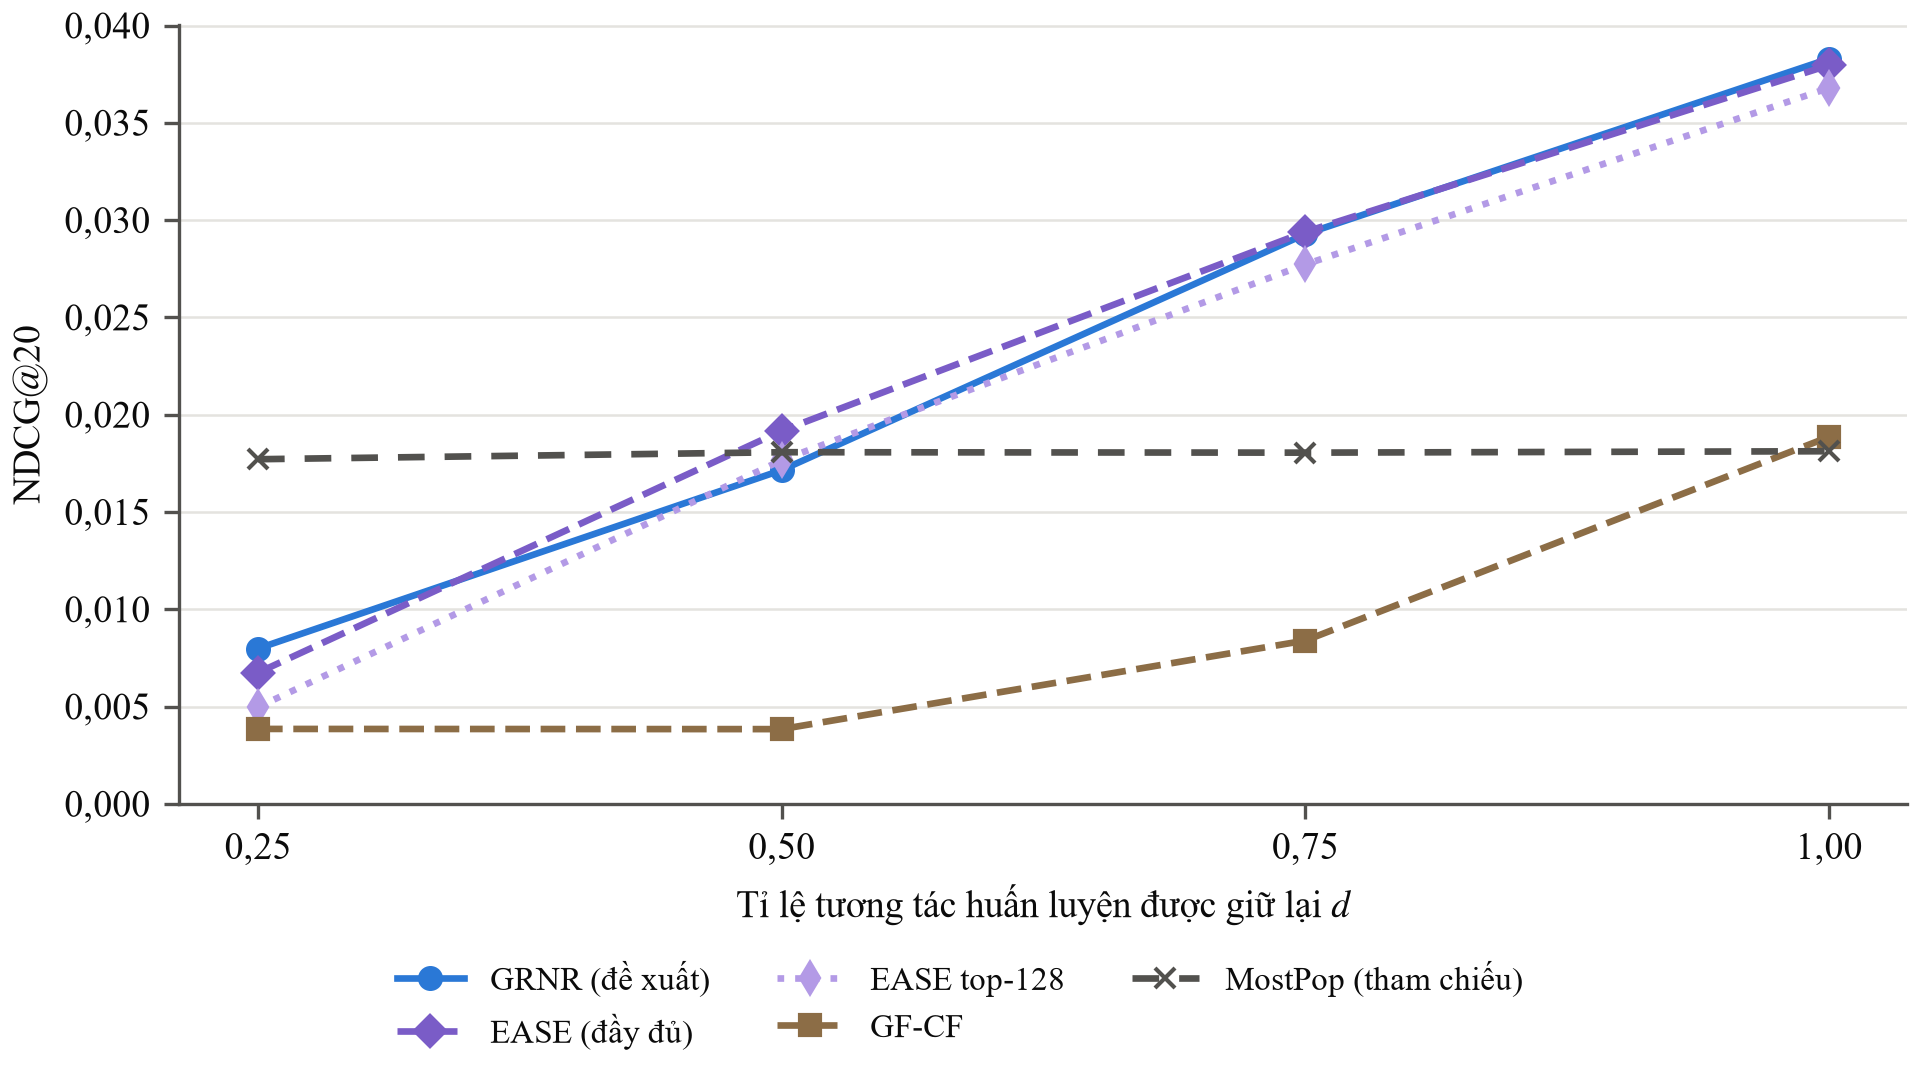
\includegraphics[width=\linewidth]{H9_mostpop_closed_ndcg20.png}
\caption[NDCG@20 của các mô hình giải trực tiếp theo tỉ lệ dữ liệu huấn luyện được giữ lại]{NDCG@20 của các mô hình giải trực tiếp theo tỉ lệ dữ liệu huấn luyện được giữ lại. Đường nét đứt là mốc MostPop, xếp hạng theo độ phổ biến trong tập huấn luyện giữ lại, không thuộc nhóm nào. Đo trên tập validation, seed 42, 107.215 người dùng có sản phẩm mục tiêu nằm trong tập ứng viên.}
\label{fig:closed-density}
\end{figure}

\figref{fig:closed-retention} biểu diễn mức giữ chất lượng của mỗi mô hình so với chính nó ở $d=1$. Khi chỉ còn 25\% tương tác, GRNR giữ 20,8\% NDCG@20 so với $d=1$, GF-CF 20,4\%, EASE đầy đủ 17,8\% và EASE top-128 13,5\%. Cả nhóm đều suy giảm mạnh. Giá trị tỉ lệ cần đọc cùng giá trị tuyệt đối: tỉ lệ của GF-CF không giảm từ $d=0{,}5$ xuống $0{,}25$ vì NDCG@20 của GF-CF ở hai mức gần như bằng nhau (0,00384 và 0,00385). Hiện tượng này, cùng việc thời gian chạy GF-CF không tăng đều theo $d$, chưa được giải thích; các run GF-CF dùng cùng cấu hình ở mọi mức.

\begin{figure}[htbp]
\centering
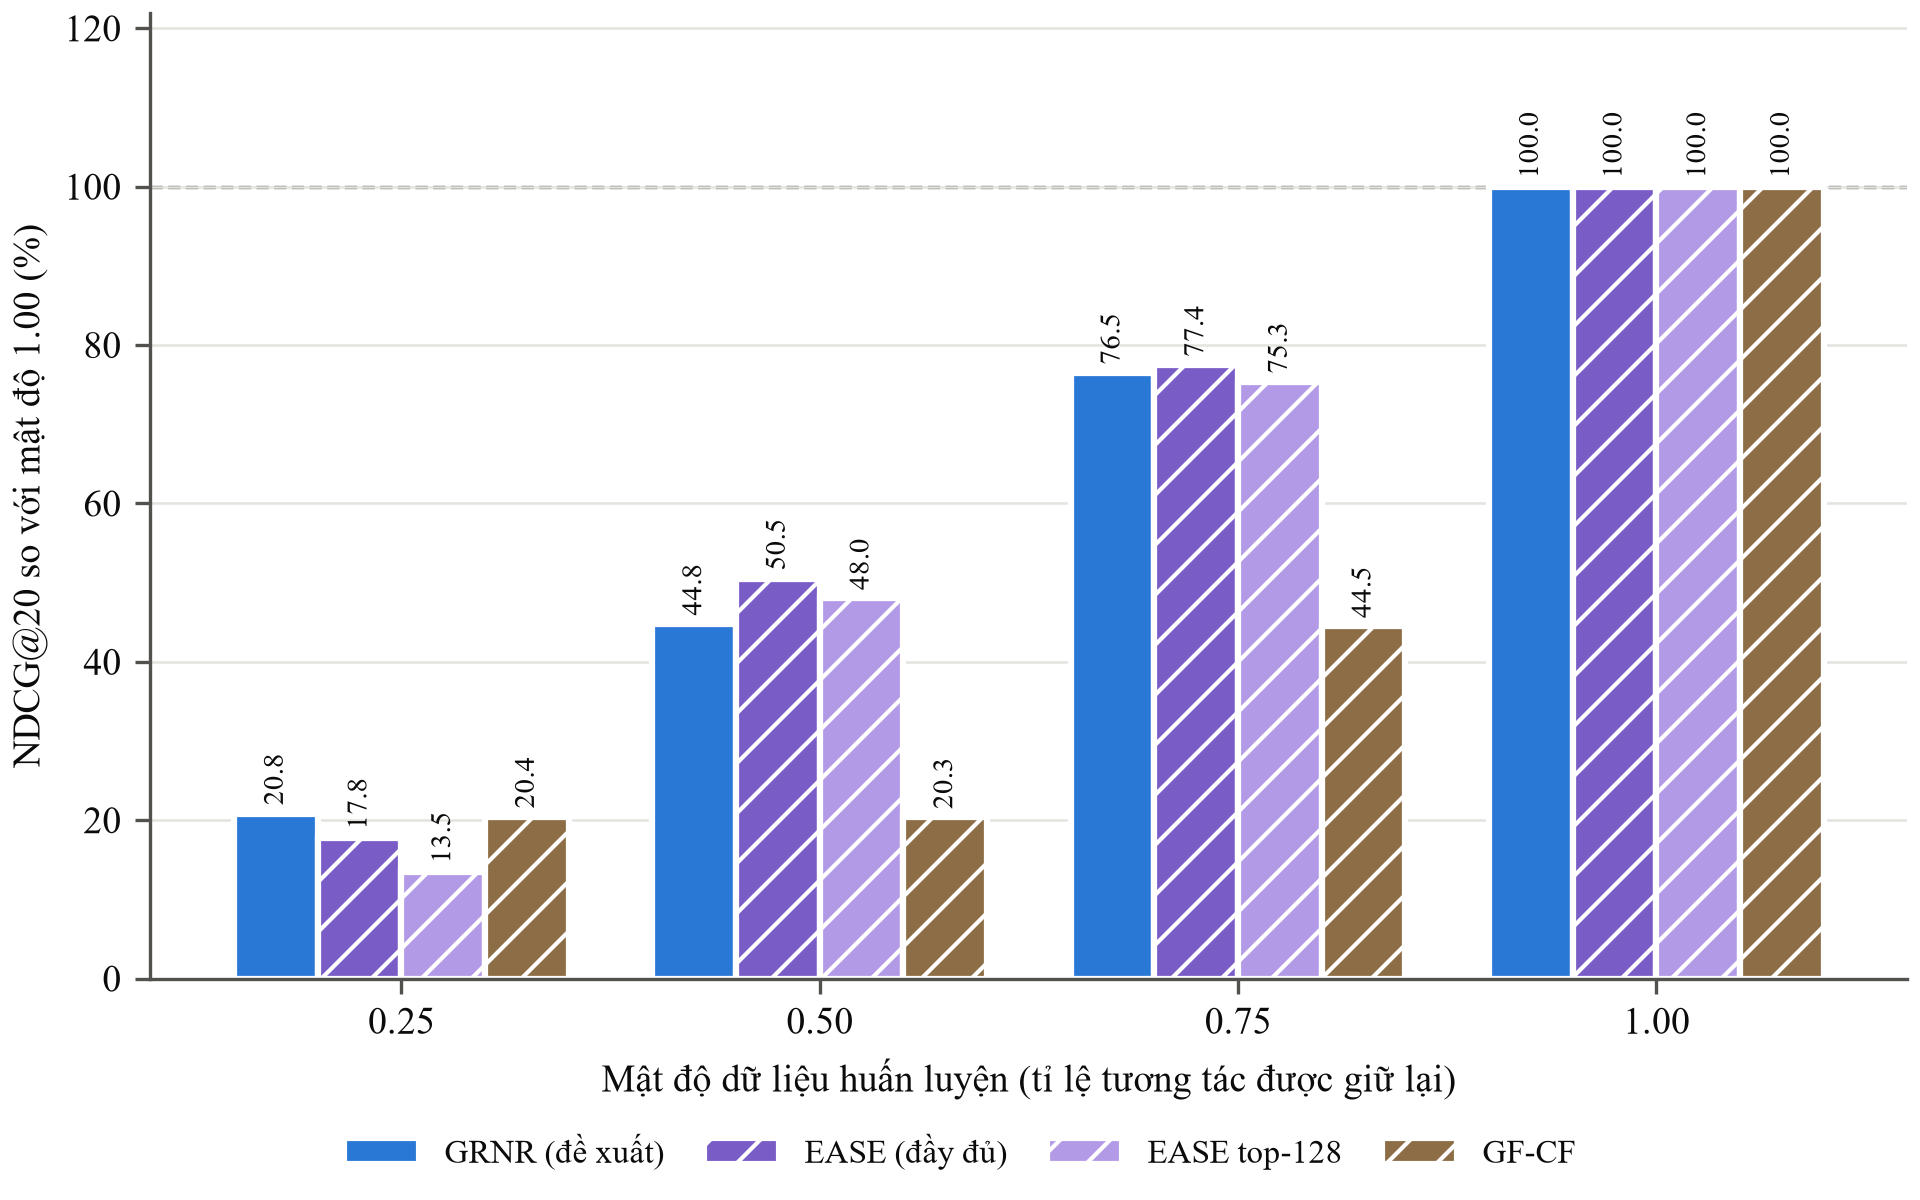
\includegraphics[width=\linewidth]{H4_closed_form_retention_ndcg20.png}
\caption[Mức giữ chất lượng của các mô hình giải trực tiếp khi giảm dữ liệu huấn luyện]{Mức giữ chất lượng của các mô hình giải trực tiếp khi giảm dữ liệu huấn luyện. NDCG@20 ở mỗi mức $d$ chia cho NDCG@20 của chính mô hình đó ở $d=1$, tính theo phần trăm.}
\label{fig:closed-retention}
\end{figure}

\figref{fig:closed-groups} chia người dùng theo số tương tác trong train gốc (3--4, 5--9, $\ge10$). Nhóm được định nghĩa theo train gốc nên giống nhau ở mọi mức $d$, và kích thước mỗi nhóm được ghi dưới trục hoành.

\begin{figure}[htbp]
\centering
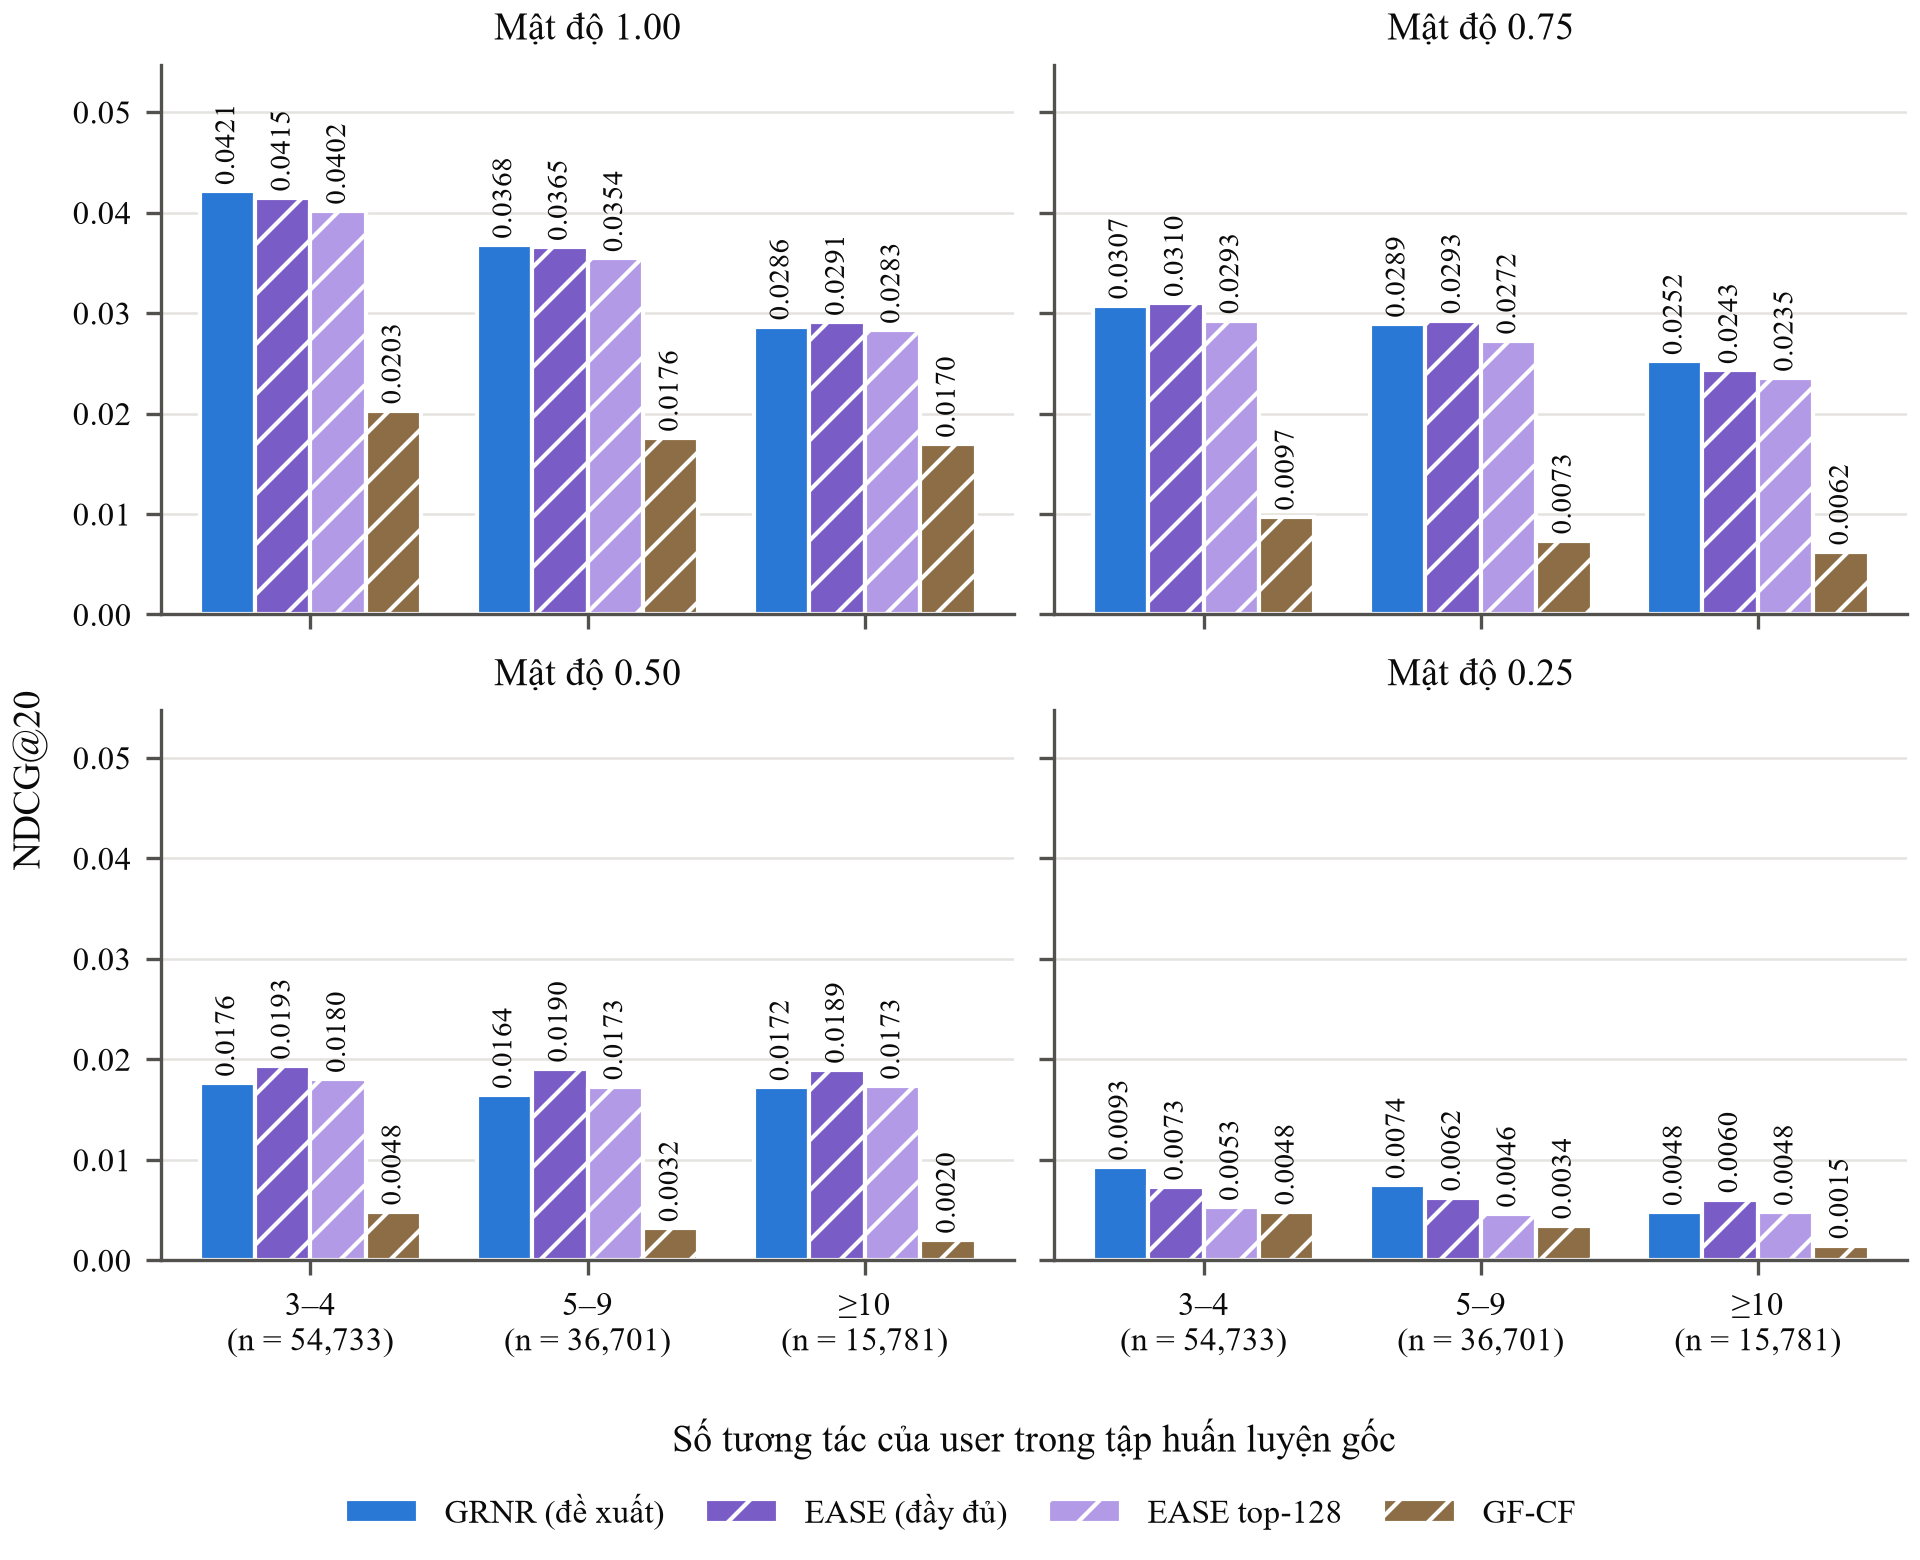
\includegraphics[width=\linewidth]{H5_closed_form_user_groups_ndcg20.png}
\caption[NDCG@20 của các mô hình giải trực tiếp theo nhóm người dùng]{NDCG@20 của các mô hình giải trực tiếp theo nhóm người dùng. Người dùng được chia theo số tương tác trong tập huấn luyện gốc; mỗi ô con ứng với một mức $d$.}
\label{fig:closed-groups}
\end{figure}

\subsubsection{Chi phí tính toán}

Ở $d=1$, GRNR mất 2,5 phút để fit và lưu checkpoint 40,5 MiB. EASE mất 11,2 phút; ma trận trọng số đầy đủ ở dạng float32 chiếm khoảng 7.671 MiB (con số ước tính, ma trận này không được lưu), còn bản cắt top-128 chiếm 31,9 MiB. GF-CF mất 45,2 phút và 43,2 MiB (\figref{fig:closed-time}, \figref{fig:closed-size}). Các run không chạy trên cùng một máy: GRNR giải trên CPU một luồng của máy có GPU, còn EASE và GF-CF chạy trên máy chỉ có CPU. Vì vậy các con số này mô tả chi phí trong môi trường của dự án, không phải so sánh tốc độ về bản chất thuật toán.

\begin{figure}[htbp]
\centering
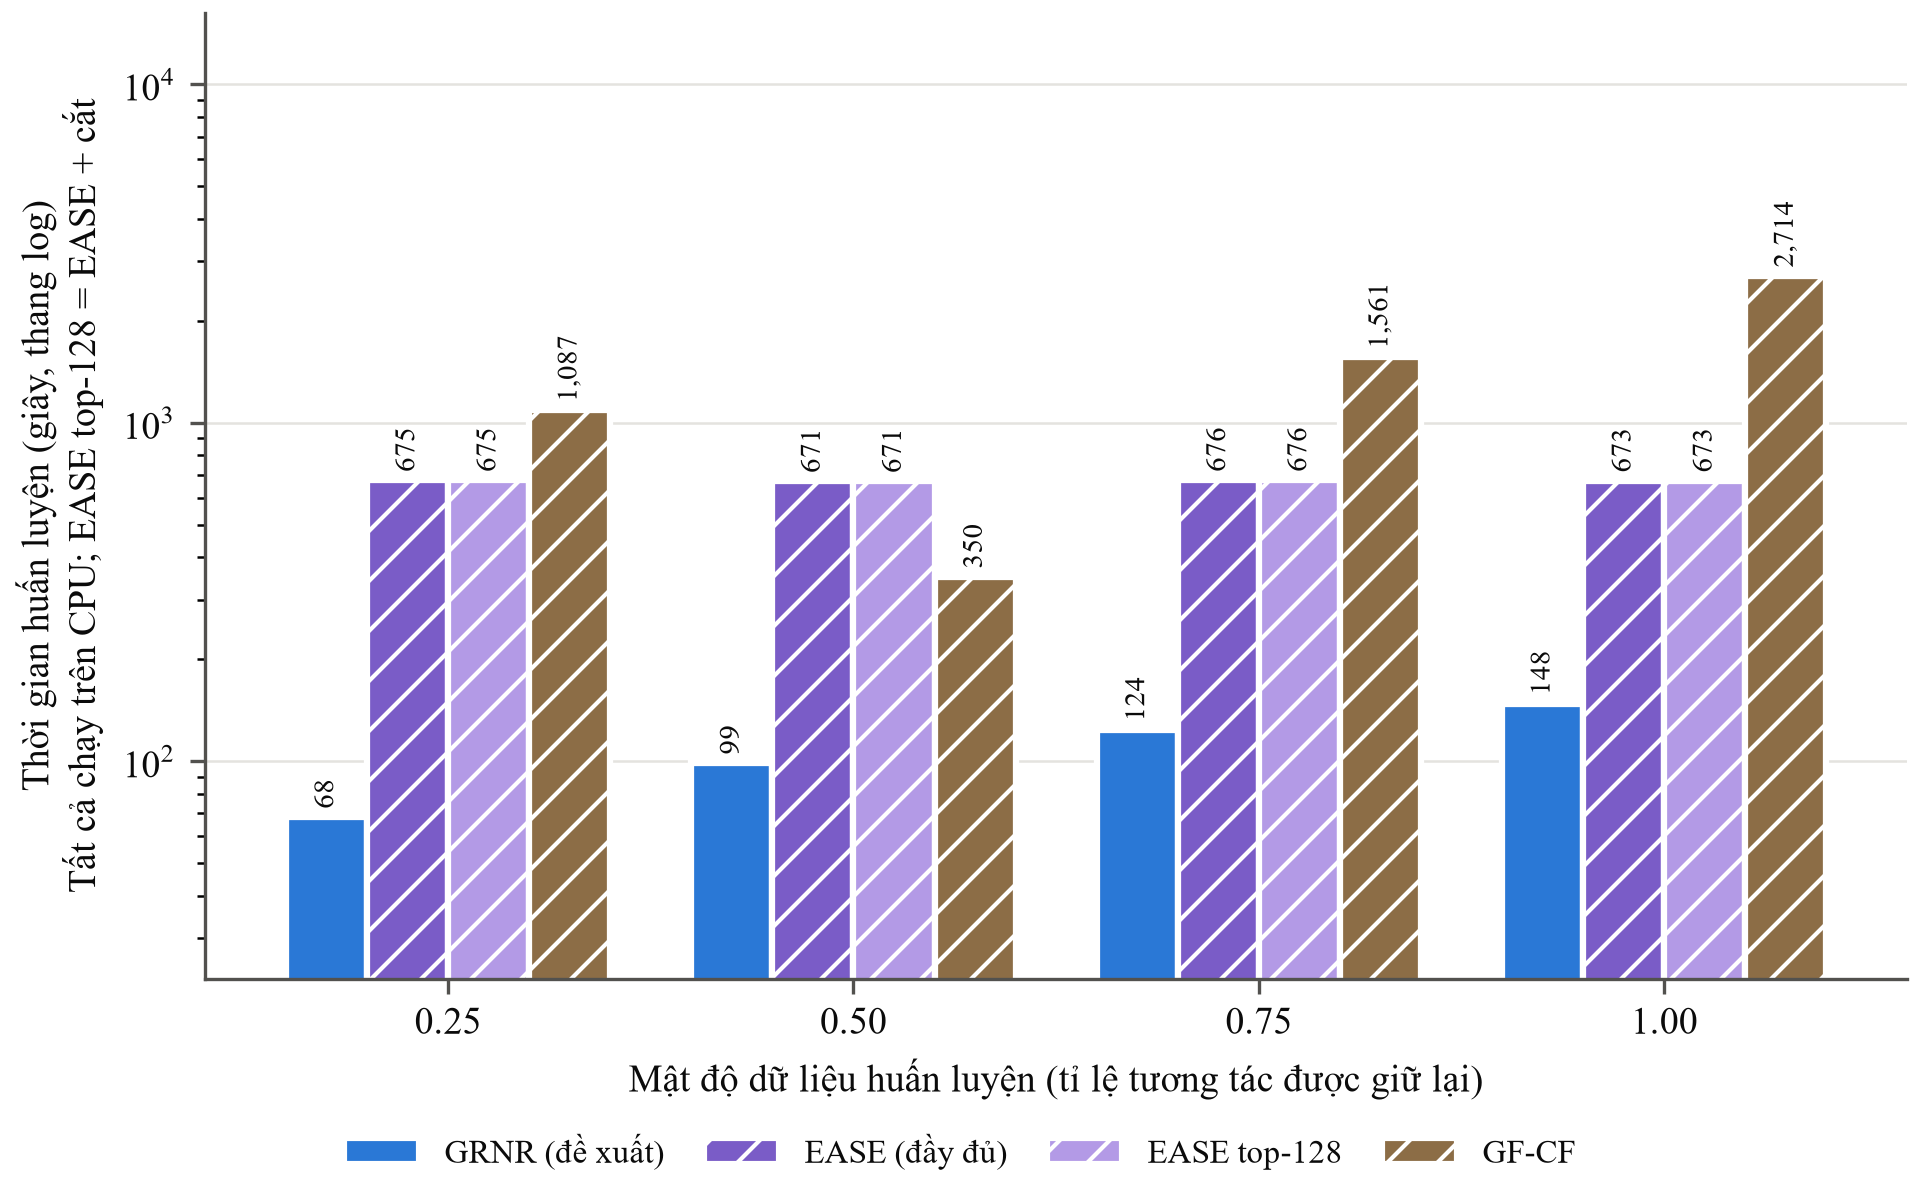
\includegraphics[width=\linewidth]{H7a_closed_form_train_time.png}
\caption[Thời gian huấn luyện của các mô hình giải trực tiếp]{Thời gian huấn luyện của các mô hình giải trực tiếp. Trục tung theo thang log, đơn vị giây; các mô hình không chạy trên cùng một máy.}
\label{fig:closed-time}
\end{figure}

\begin{figure}[htbp]
\centering
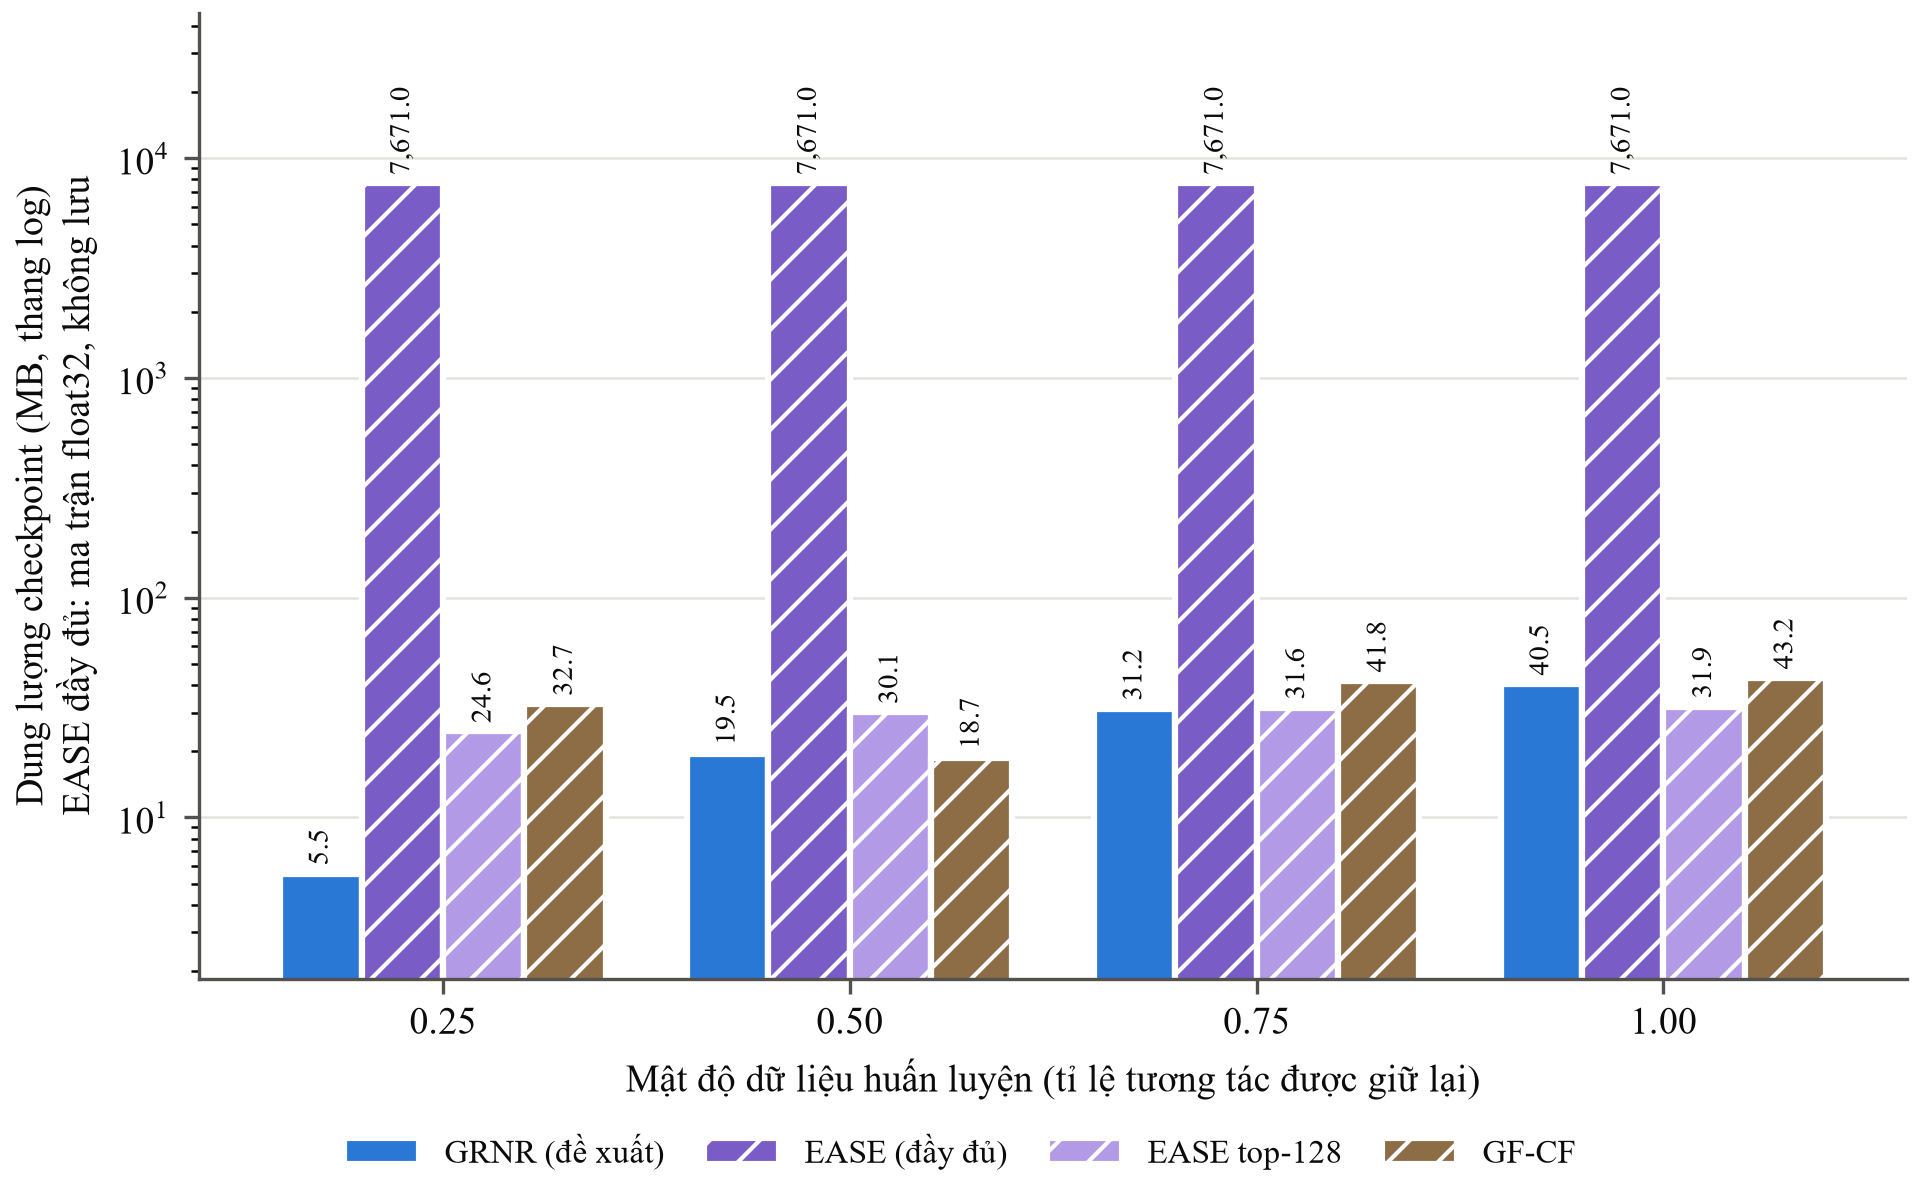
\includegraphics[width=\linewidth]{H7c_closed_form_checkpoint_size.png}
\caption[Dung lượng lưu trữ của các mô hình giải trực tiếp]{Dung lượng lưu trữ của các mô hình giải trực tiếp. Trục tung theo thang log, đơn vị MiB. Với EASE đầy đủ, đây là kích thước ước tính của ma trận float32, không phải tệp đã lưu.}
\label{fig:closed-size}
\end{figure}

\subsection{Diffusion-Filtered History Factorization so với các mô hình cần huấn luyện}
\label{sec:dfhf-results}

\subsubsection{Chất lượng xếp hạng}

\tabref{tab:trained} cho kết quả của nhóm cần huấn luyện. Ở $d=1$, DFHF đạt NDCG@20 bằng 0,03519, cao hơn XSimGCL (0,03292), DirectAU (0,03205) và LightGCN (0,02655). Theo \tabref{tab:trained-sig}, cả ba chênh lệch đều dương với khoảng tin cậy không chứa 0: so với XSimGCL $\Delta=+0{,}00228$ (KTC $[0{,}00172;\,0{,}00284]$), so với DirectAU $\Delta=+0{,}00314$, so với LightGCN $\Delta=+0{,}00864$.

\begin{table}[htbp]
\centering
\caption[Chất lượng xếp hạng của các mô hình cần huấn luyện]{Chất lượng xếp hạng của các mô hình cần huấn luyện. Đo trên tập validation, seed 42; giá trị cao nhất ở mỗi mức $d$ được in đậm.}
\label{tab:trained}
\begin{tabular}{@{}llrrrr@{}}
\toprule
$d$ & Mô hình & NDCG@10 & NDCG@20 & Recall@10 & Recall@20 \\
\midrule
\multirow{4}{*}{1} & DFHF & \textbf{0,02946} & \textbf{0,03519} & \textbf{0,05217} & \textbf{0,07500} \\
 & LightGCN & 0,02173 & 0,02655 & 0,03998 & 0,05912 \\
 & XSimGCL & 0,02721 & 0,03292 & 0,04905 & 0,07173 \\
 & DirectAU & 0,02666 & 0,03205 & 0,04781 & 0,06925 \\
\midrule
\multirow{4}{*}{0,75} & DFHF & \textbf{0,02400} & \textbf{0,02901} & \textbf{0,04269} & \textbf{0,06261} \\
 & LightGCN & 0,01814 & 0,02261 & 0,03346 & 0,05122 \\
 & XSimGCL & 0,02288 & 0,02759 & 0,04077 & 0,05948 \\
 & DirectAU & 0,02238 & 0,02698 & 0,03960 & 0,05789 \\
\midrule
\multirow{4}{*}{0,5} & DFHF & \textbf{0,01824} & \textbf{0,02266} & \textbf{0,03377} & \textbf{0,05133} \\
 & LightGCN & 0,01455 & 0,01839 & 0,02764 & 0,04298 \\
 & XSimGCL & 0,01596 & 0,01933 & 0,02881 & 0,04223 \\
 & DirectAU & 0,01700 & 0,02050 & 0,03022 & 0,04418 \\
\midrule
\multirow{4}{*}{0,25} & DFHF & \textbf{0,01359} & \textbf{0,01766} & \textbf{0,02608} & \textbf{0,04220} \\
 & LightGCN & 0,00676 & 0,00842 & 0,01199 & 0,01857 \\
 & XSimGCL & 0,00913 & 0,01117 & 0,01725 & 0,02535 \\
 & DirectAU & 0,00849 & 0,01029 & 0,01517 & 0,02235 \\
\bottomrule
\end{tabular}
\end{table}

\begin{table}[htbp]
\centering
\caption[Kiểm định chênh lệch NDCG@20 trong nhóm cần huấn luyện]{Kiểm định chênh lệch NDCG@20 trong nhóm cần huấn luyện. Hiệu của DFHF trừ từng baseline; bootstrap ghép cặp theo người dùng 10.000 lần ($n=107.215$); giá trị $p$ một phía, hiệu chỉnh Holm trong mỗi mức $d$. Phân tích được thực hiện sau khi đã xem điểm trung bình, nên mang tính khám phá.}
\label{tab:trained-sig}
\begin{tabular}{@{}llrrr@{}}
\toprule
$d$ & So sánh & $\Delta$ NDCG@20 & KTC 95\% & $p_{\mathrm{Holm}}$ (một phía) \\
\midrule
\multirow{3}{*}{1} & DFHF $-$ LightGCN & $+0{,}00864$ & $[+0{,}00802;\;+0{,}00928]$ & $\le 3\cdot10^{-4}$ \\
 & DFHF $-$ XSimGCL & $+0{,}00228$ & $[+0{,}00172;\;+0{,}00284]$ & $\le 3\cdot10^{-4}$ \\
 & DFHF $-$ DirectAU & $+0{,}00314$ & $[+0{,}00251;\;+0{,}00378]$ & $\le 3\cdot10^{-4}$ \\
\midrule
\multirow{3}{*}{0,75} & DFHF $-$ LightGCN & $+0{,}00640$ & $[+0{,}00582;\;+0{,}00699]$ & $\le 3\cdot10^{-4}$ \\
 & DFHF $-$ XSimGCL & $+0{,}00142$ & $[+0{,}00086;\;+0{,}00201]$ & $\le 3\cdot10^{-4}$ \\
 & DFHF $-$ DirectAU & $+0{,}00203$ & $[+0{,}00142;\;+0{,}00266]$ & $\le 3\cdot10^{-4}$ \\
\midrule
\multirow{3}{*}{0,5} & DFHF $-$ LightGCN & $+0{,}00427$ & $[+0{,}00376;\;+0{,}00479]$ & $\le 3\cdot10^{-4}$ \\
 & DFHF $-$ XSimGCL & $+0{,}00333$ & $[+0{,}00273;\;+0{,}00392]$ & $\le 3\cdot10^{-4}$ \\
 & DFHF $-$ DirectAU & $+0{,}00216$ & $[+0{,}00152;\;+0{,}00281]$ & $\le 3\cdot10^{-4}$ \\
\midrule
\multirow{3}{*}{0,25} & DFHF $-$ LightGCN & $+0{,}00924$ & $[+0{,}00867;\;+0{,}00982]$ & $\le 3\cdot10^{-4}$ \\
 & DFHF $-$ XSimGCL & $+0{,}00649$ & $[+0{,}00596;\;+0{,}00706]$ & $\le 3\cdot10^{-4}$ \\
 & DFHF $-$ DirectAU & $+0{,}00737$ & $[+0{,}00674;\;+0{,}00802]$ & $\le 3\cdot10^{-4}$ \\
\bottomrule
\end{tabular}
\end{table}

Các chênh lệch này cần được đọc cùng hai giới hạn của giao thức. Thứ nhất, mọi mô hình trong nhóm đều được chọn checkpoint trên chính tập validation dùng để báo cáo. Thứ hai, DirectAU đạt điểm cao nhất ở epoch cuối cùng (200/200) tại $d=1$, và ở epoch 195 và 181 tại $d=0{,}5$ và $d=0{,}25$, nên có thể chưa hội tụ trong giới hạn 200 epoch; chênh lệch giữa DFHF và DirectAU vì thế có thể bị phóng đại.

\subsubsection{Ảnh hưởng của mức độ thưa và nhóm người dùng}

DFHF có NDCG@20 cao nhất nhóm ở cả bốn mức $d$ (\figref{fig:trained-density}), và theo \tabref{tab:trained-sig} chênh lệch với cả ba baseline đều có khoảng tin cậy không chứa 0 ở mọi mức. Chênh lệch lớn nhất ở $d=0{,}25$: 0,01766 so với 0,01117 của XSimGCL. Tuy nhiên, đường MostPop trong hình cho thấy ở $d=0{,}25$ DFHF chỉ ngang xếp hạng theo độ phổ biến, còn ba baseline đều thấp hơn mốc này; ở $d=0{,}5$, LightGCN cũng chỉ xấp xỉ MostPop. Phần cuối mục này giải thích vì sao.

\begin{figure}[htbp]
\centering
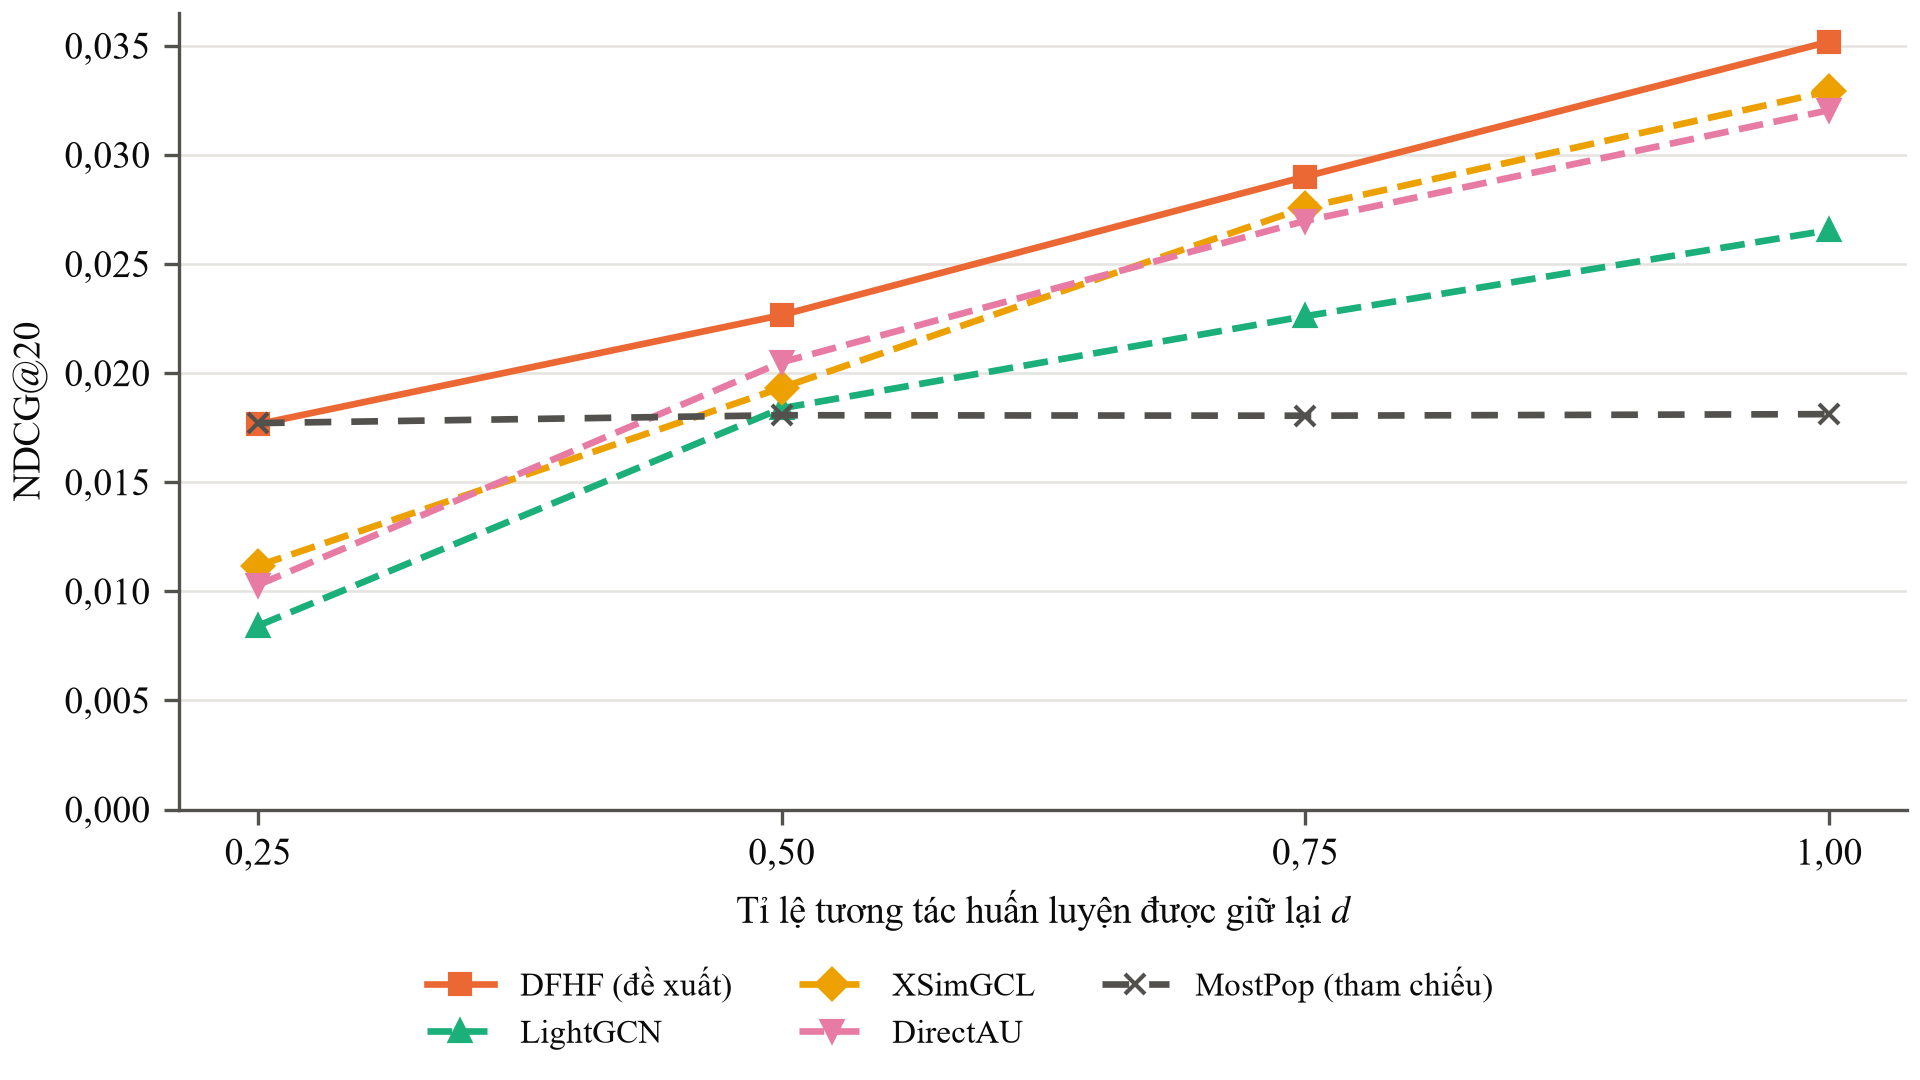
\includegraphics[width=\linewidth]{H9_mostpop_trained_ndcg20.png}
\caption[NDCG@20 của các mô hình cần huấn luyện theo tỉ lệ dữ liệu huấn luyện được giữ lại]{NDCG@20 của các mô hình cần huấn luyện theo tỉ lệ dữ liệu huấn luyện được giữ lại. Đường nét đứt là mốc MostPop, xếp hạng theo độ phổ biến trong tập huấn luyện giữ lại, không thuộc nhóm nào. Đo trên tập validation, seed 42, 107.215 người dùng có sản phẩm mục tiêu nằm trong tập ứng viên.}
\label{fig:trained-density}
\end{figure}

Về mức giữ chất lượng (\figref{fig:trained-retention}), ở $d=0{,}25$ DFHF giữ 50,2\% NDCG@20 so với $d=1$, cao hơn XSimGCL (33,9\%), DirectAU (32,1\%) và LightGCN (31,7\%). Tuy nhiên DFHF không giữ chất lượng tốt nhất ở mọi mức: ở $d=0{,}5$, LightGCN giữ 69,3\%, cao hơn DFHF (64,4\%), DirectAU (64,0\%) và XSimGCL (58,7\%).

\begin{figure}[htbp]
\centering
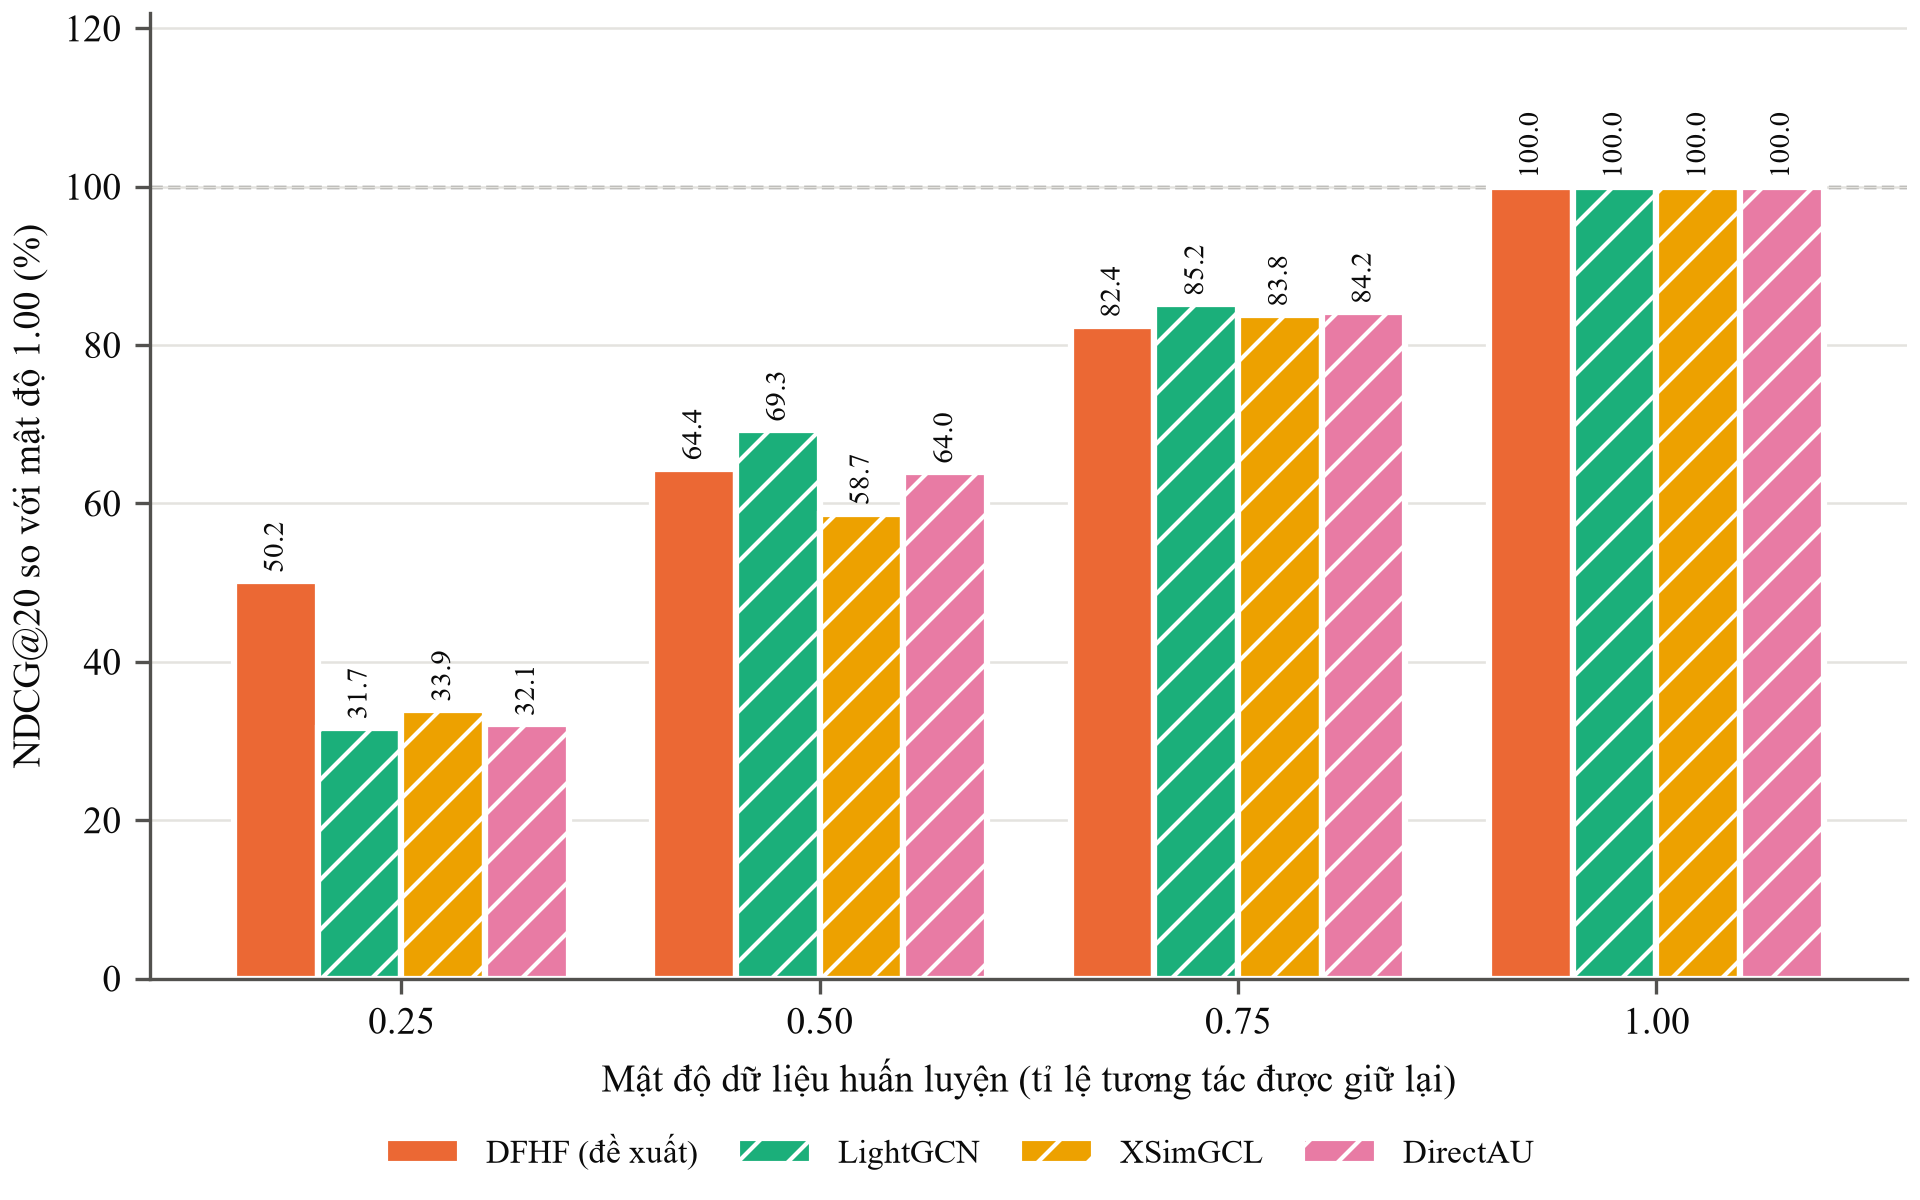
\includegraphics[width=\linewidth]{H4_trained_retention_ndcg20.png}
\caption[Mức giữ chất lượng của các mô hình cần huấn luyện khi giảm dữ liệu huấn luyện]{Mức giữ chất lượng của các mô hình cần huấn luyện khi giảm dữ liệu huấn luyện. NDCG@20 ở mỗi mức $d$ chia cho NDCG@20 của chính mô hình đó ở $d=1$, tính theo phần trăm.}
\label{fig:trained-retention}
\end{figure}

Kết quả ở $d=0{,}25$ cần được diễn giải thận trọng. Như đã nêu ở Mục~\ref{sec:dfhf-representation}, DFHF xếp hạng những người dùng chỉ còn một tương tác bằng vector chặn $b$, tức một thứ tự độ phổ biến đã học. Ở $d=0{,}25$, nhóm này chiếm 68\% người dùng warm. Tách kết quả theo bậc người dùng (\tabref{tab:degree-split}) cho thấy DFHF đạt 0,01787 trên người dùng bậc 1, gần như trùng với một xếp hạng theo độ phổ biến thuần túy (0,01789). Mục~\ref{sec:discussion} phân tích hệ quả của quan sát này.

\begin{table}[htbp]
\centering
\caption[NDCG@20 của các mô hình cần huấn luyện theo số tương tác còn lại]{NDCG@20 của các mô hình cần huấn luyện theo số tương tác còn lại. Ở mức $d=0{,}25$. MostPop là mốc tham chiếu xếp hạng theo độ phổ biến, không thuộc nhóm nào.}
\label{tab:degree-split}
\begin{tabular}{@{}lrrr@{}}
\toprule
Mô hình & Bậc 1 ($n=72.944$) & Bậc $\ge2$ ($n=34.271$) & Tất cả \\
\midrule
DFHF & 0,01787 & 0,01720 & 0,01766 \\
LightGCN & 0,00849 & 0,00826 & 0,00842 \\
XSimGCL & 0,01132 & 0,01084 & 0,01117 \\
DirectAU & 0,01023 & 0,01043 & 0,01029 \\
\midrule
MostPop (tham chiếu) & 0,01789 & 0,01733 & 0,01771 \\
\bottomrule
\end{tabular}
\end{table}

\figref{fig:trained-groups} chia người dùng theo số tương tác trong train gốc. Ở $d=1$, DFHF cao nhất ở nhóm 3--4 và 5--9 tương tác, còn ở nhóm $\ge10$ tương tác XSimGCL nhỉnh hơn (0,0235 so với 0,0230).

\begin{figure}[htbp]
\centering
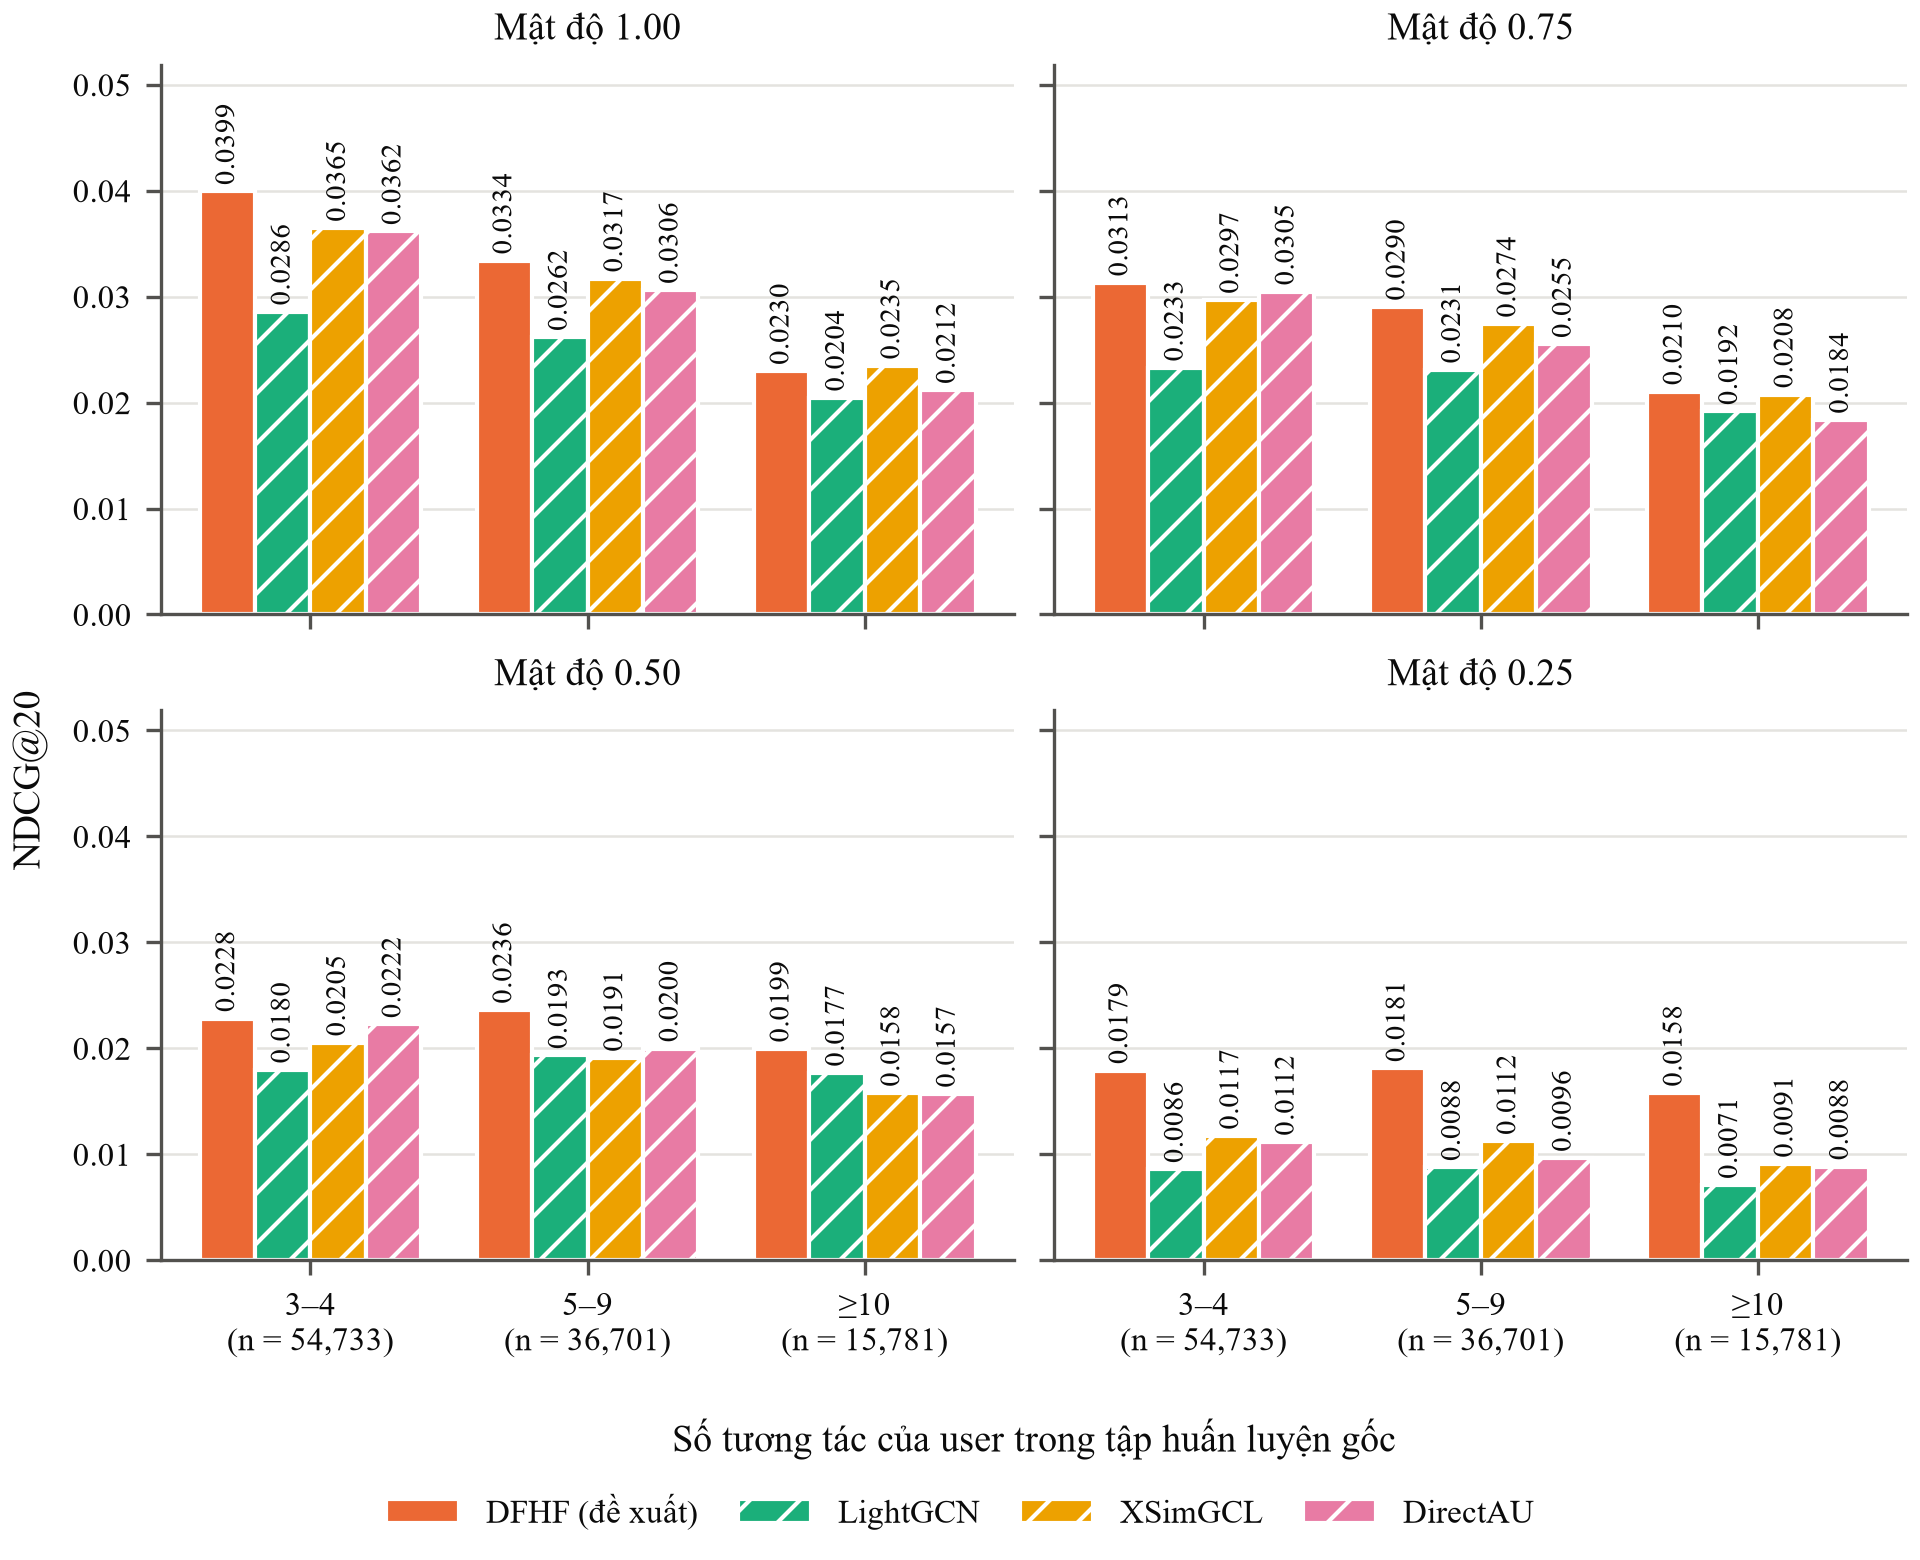
\includegraphics[width=\linewidth]{H5_trained_user_groups_ndcg20.png}
\caption[NDCG@20 của các mô hình cần huấn luyện theo nhóm người dùng]{NDCG@20 của các mô hình cần huấn luyện theo nhóm người dùng. Người dùng được chia theo số tương tác trong tập huấn luyện gốc; mỗi ô con ứng với một mức $d$.}
\label{fig:trained-groups}
\end{figure}

\subsubsection{Quá trình huấn luyện và chi phí tính toán}

\figref{fig:trained-curves} vẽ NDCG@20 validation theo epoch; dấu đánh dấu là epoch được chọn. DFHF đạt đỉnh ở epoch 71 tại $d=1$ rồi giảm dần, đến epoch 200 còn 0,02658, thấp hơn đỉnh 24,5\% (\tabref{tab:training}). XSimGCL có hiện tượng tương tự (giảm 21,4\%), trong khi LightGCN và DirectAU gần như không giảm. Như vậy kết quả của DFHF và XSimGCL phụ thuộc nhiều vào việc chọn checkpoint trên validation.

\begin{figure}[htbp]
\centering
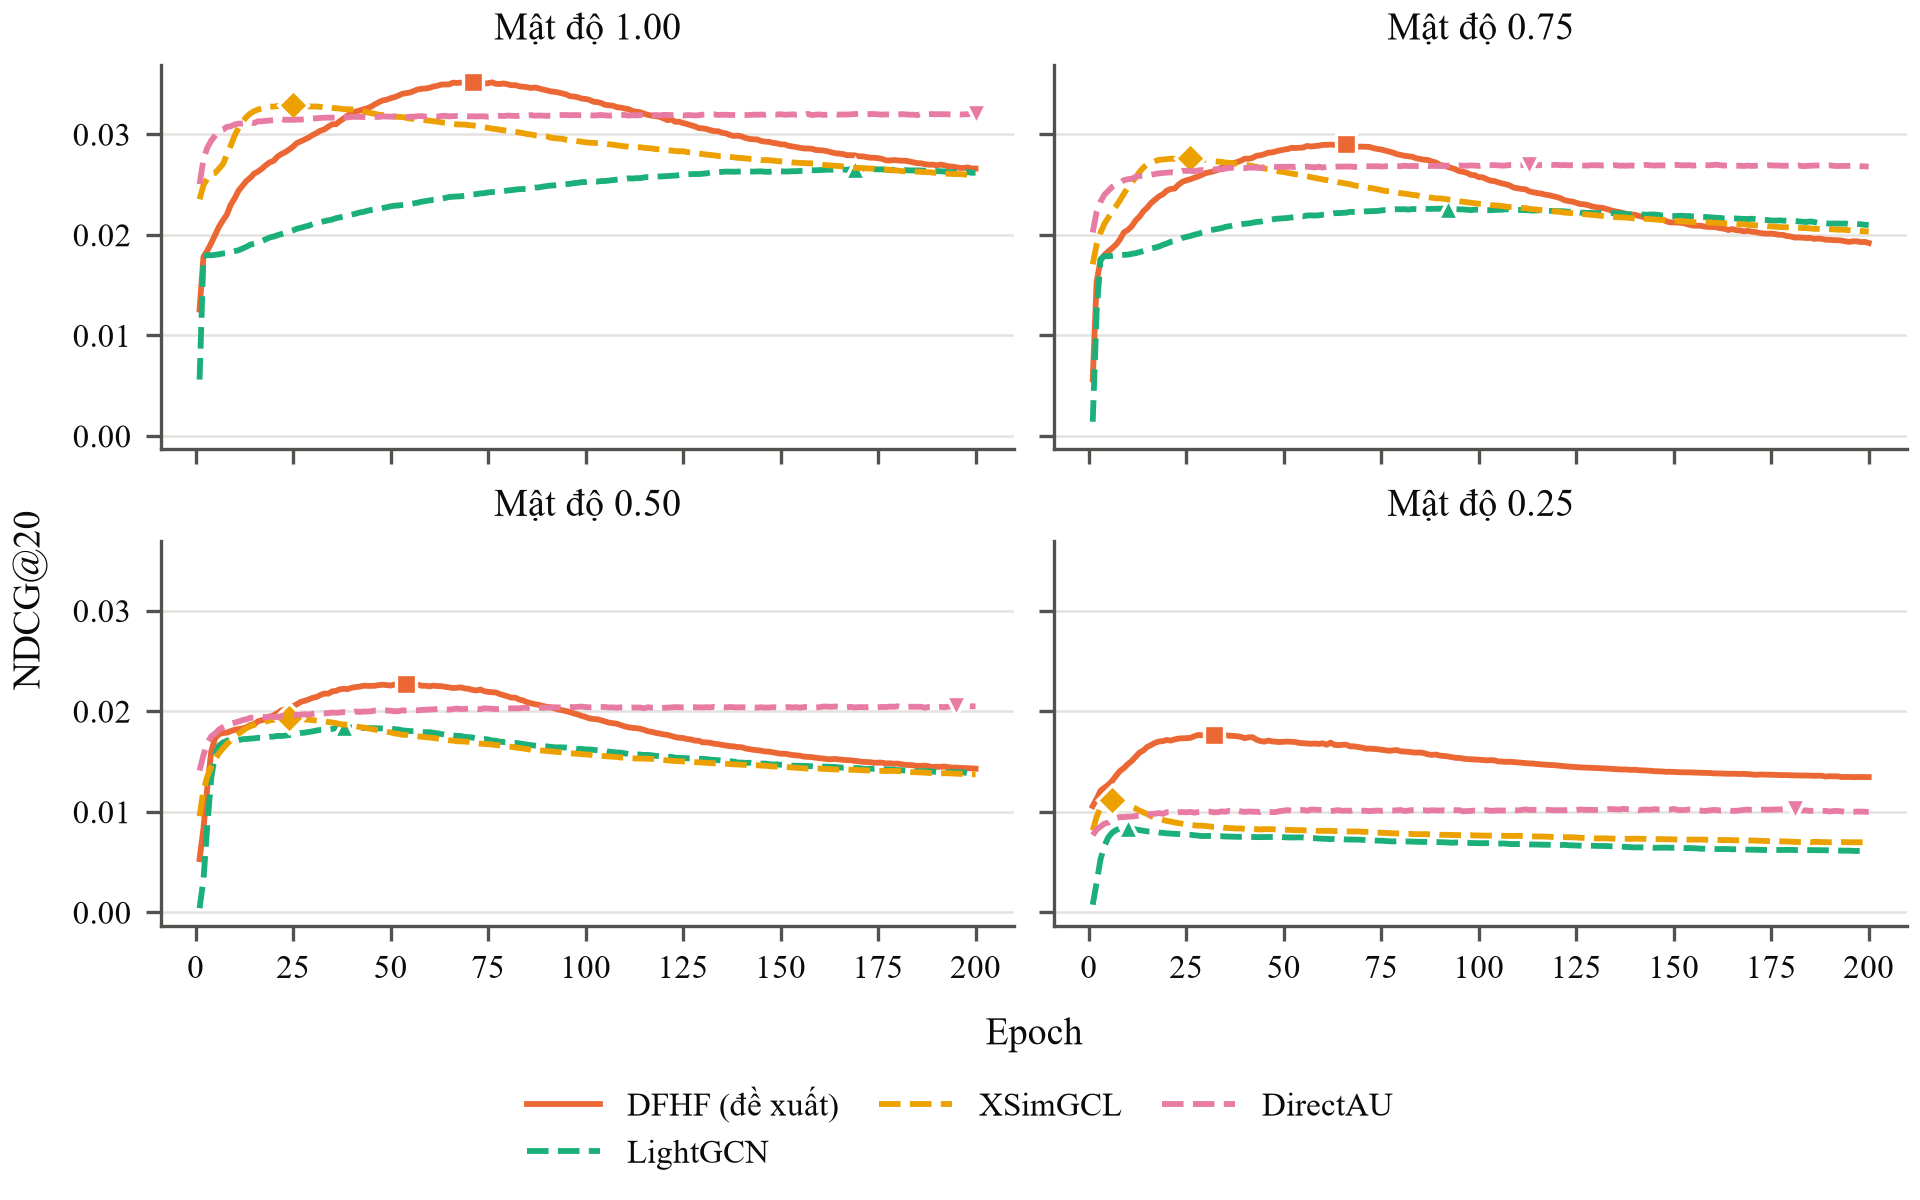
\includegraphics[width=\linewidth]{H3_trained_learning_curves_ndcg20.png}
\caption[Đường học của các mô hình cần huấn luyện]{Đường học của các mô hình cần huấn luyện. NDCG@20 trên tập validation theo epoch ở bốn mức $d$; dấu đánh dấu là epoch được chọn làm checkpoint.}
\label{fig:trained-curves}
\end{figure}

\begin{table}[htbp]
\centering
\caption[Quá trình huấn luyện và chi phí của các mô hình cần huấn luyện]{Quá trình huấn luyện và chi phí của các mô hình cần huấn luyện. Ở mức $d=1$: epoch được chọn làm checkpoint, mức giảm NDCG@20 đến epoch cuối và thời gian mỗi epoch trên GPU Tesla T4.}
\label{tab:training}
\begin{tabular}{@{}lrrrrr@{}}
\toprule
Mô hình & Epoch chọn & NDCG@20 chọn & NDCG@20 cuối & Giảm & Giây/epoch \\
\midrule
DFHF & 71 & 0,03519 & 0,02658 & 24,5\% & 37,9 \\
LightGCN & 169 & 0,02655 & 0,02617 & 1,4\% & 11,2 \\
XSimGCL & 25 & 0,03292 & 0,02587 & 21,4\% & 17,7 \\
DirectAU & 200 & 0,03205 & 0,03205 & 0\% & 24,1 \\
\bottomrule
\end{tabular}
\end{table}

Về chi phí, DFHF là mô hình chậm nhất nhóm: 37,9 giây mỗi epoch, tổng khoảng 127 phút cho 200 epoch ở $d=1$, so với 24,1 giây của DirectAU, 17,7 giây của XSimGCL và 11,2 giây của LightGCN (\figref{fig:trained-time}). Phần lớn chi phí đến từ softmax trên toàn bộ danh mục và hai lần áp toán tử khuếch tán ở mỗi bước. Khi suy luận, cả bốn mô hình đều mất khoảng 0,01 ms cho mỗi người dùng theo lô trên GPU (\figref{fig:trained-latency}). Đây là trung bình theo lô, không phải độ trễ của một dịch vụ thực tế.

\begin{figure}[htbp]
\centering
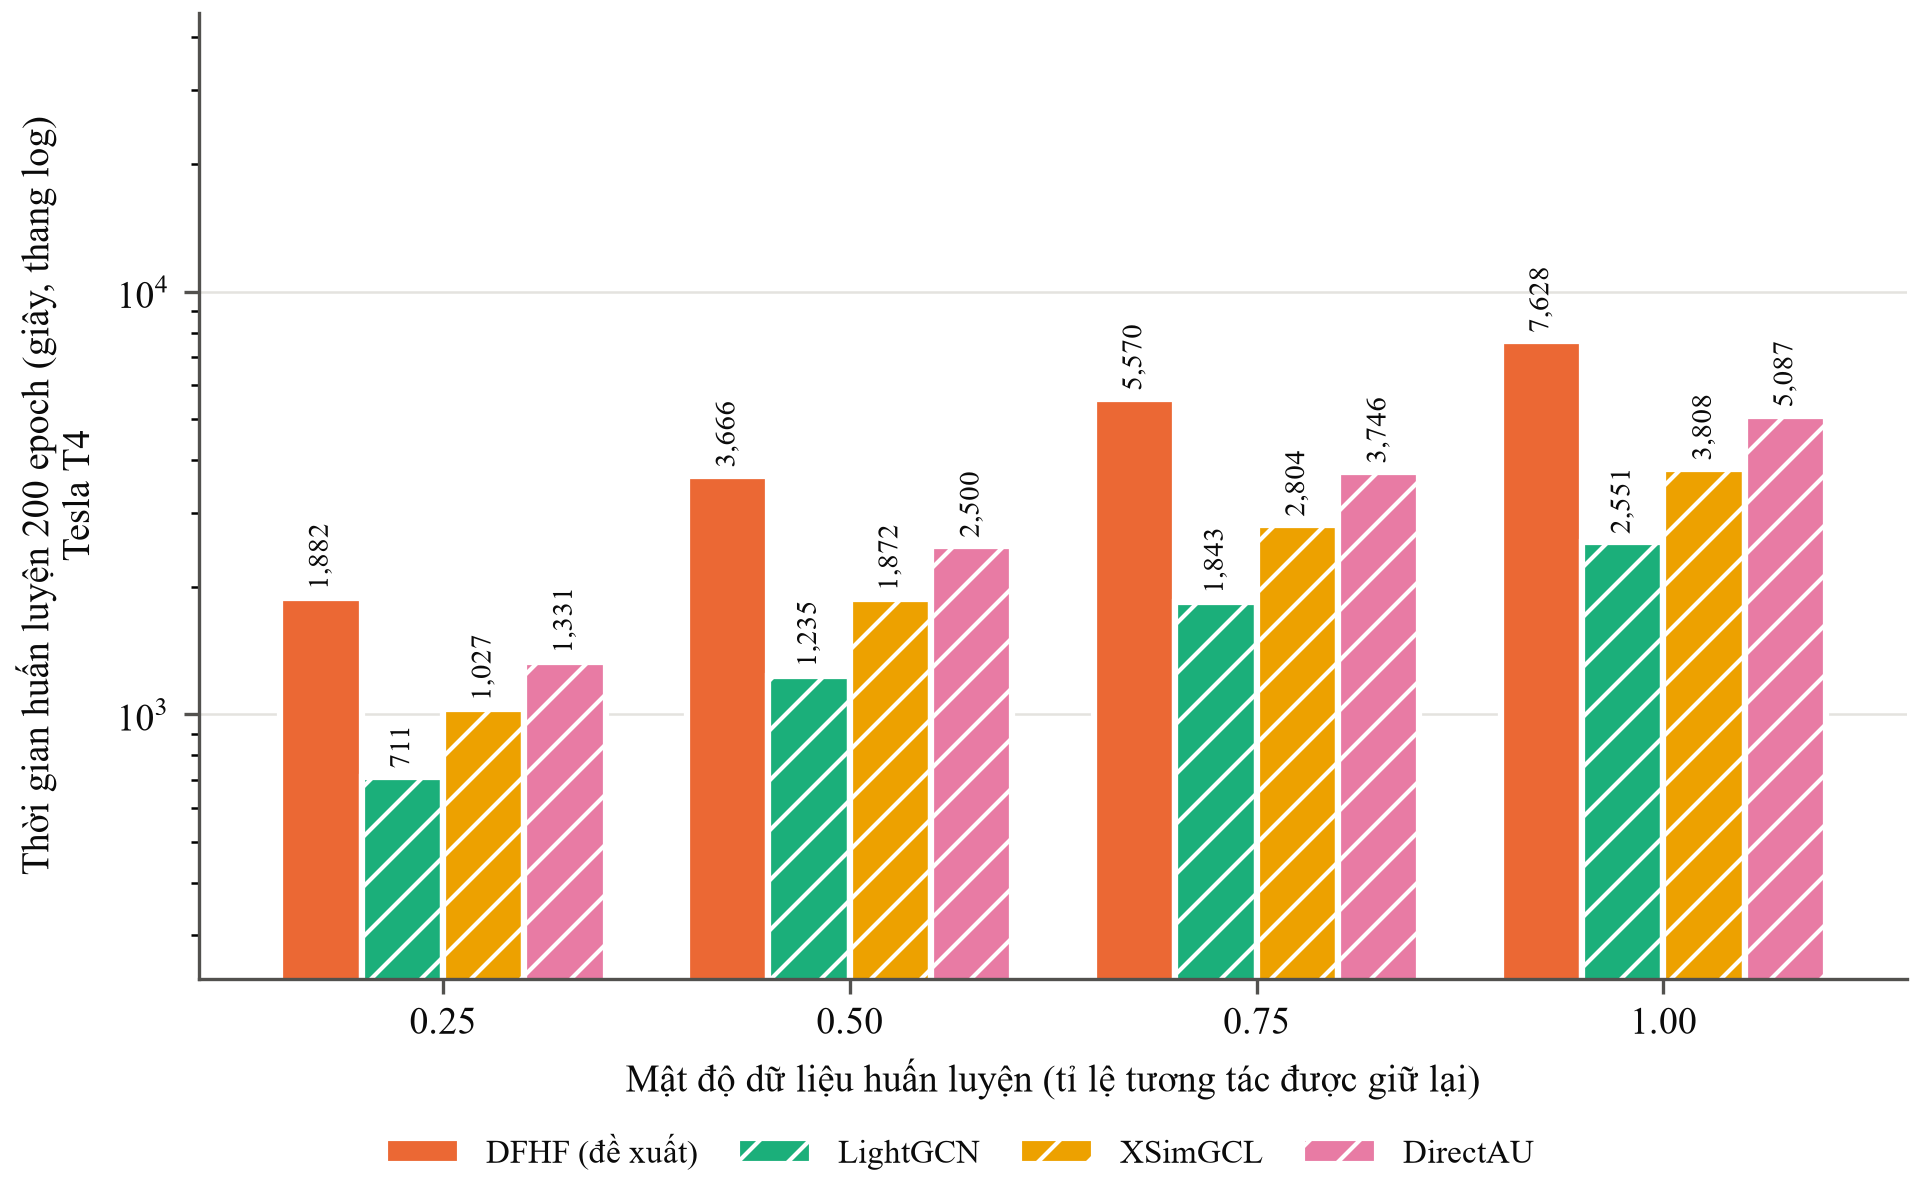
\includegraphics[width=\linewidth]{H7a_trained_train_time.png}
\caption[Thời gian huấn luyện của các mô hình cần huấn luyện]{Thời gian huấn luyện của các mô hình cần huấn luyện. Tổng thời gian 200 epoch trên GPU Tesla T4; trục tung theo thang log, đơn vị giây.}
\label{fig:trained-time}
\end{figure}

\begin{figure}[htbp]
\centering
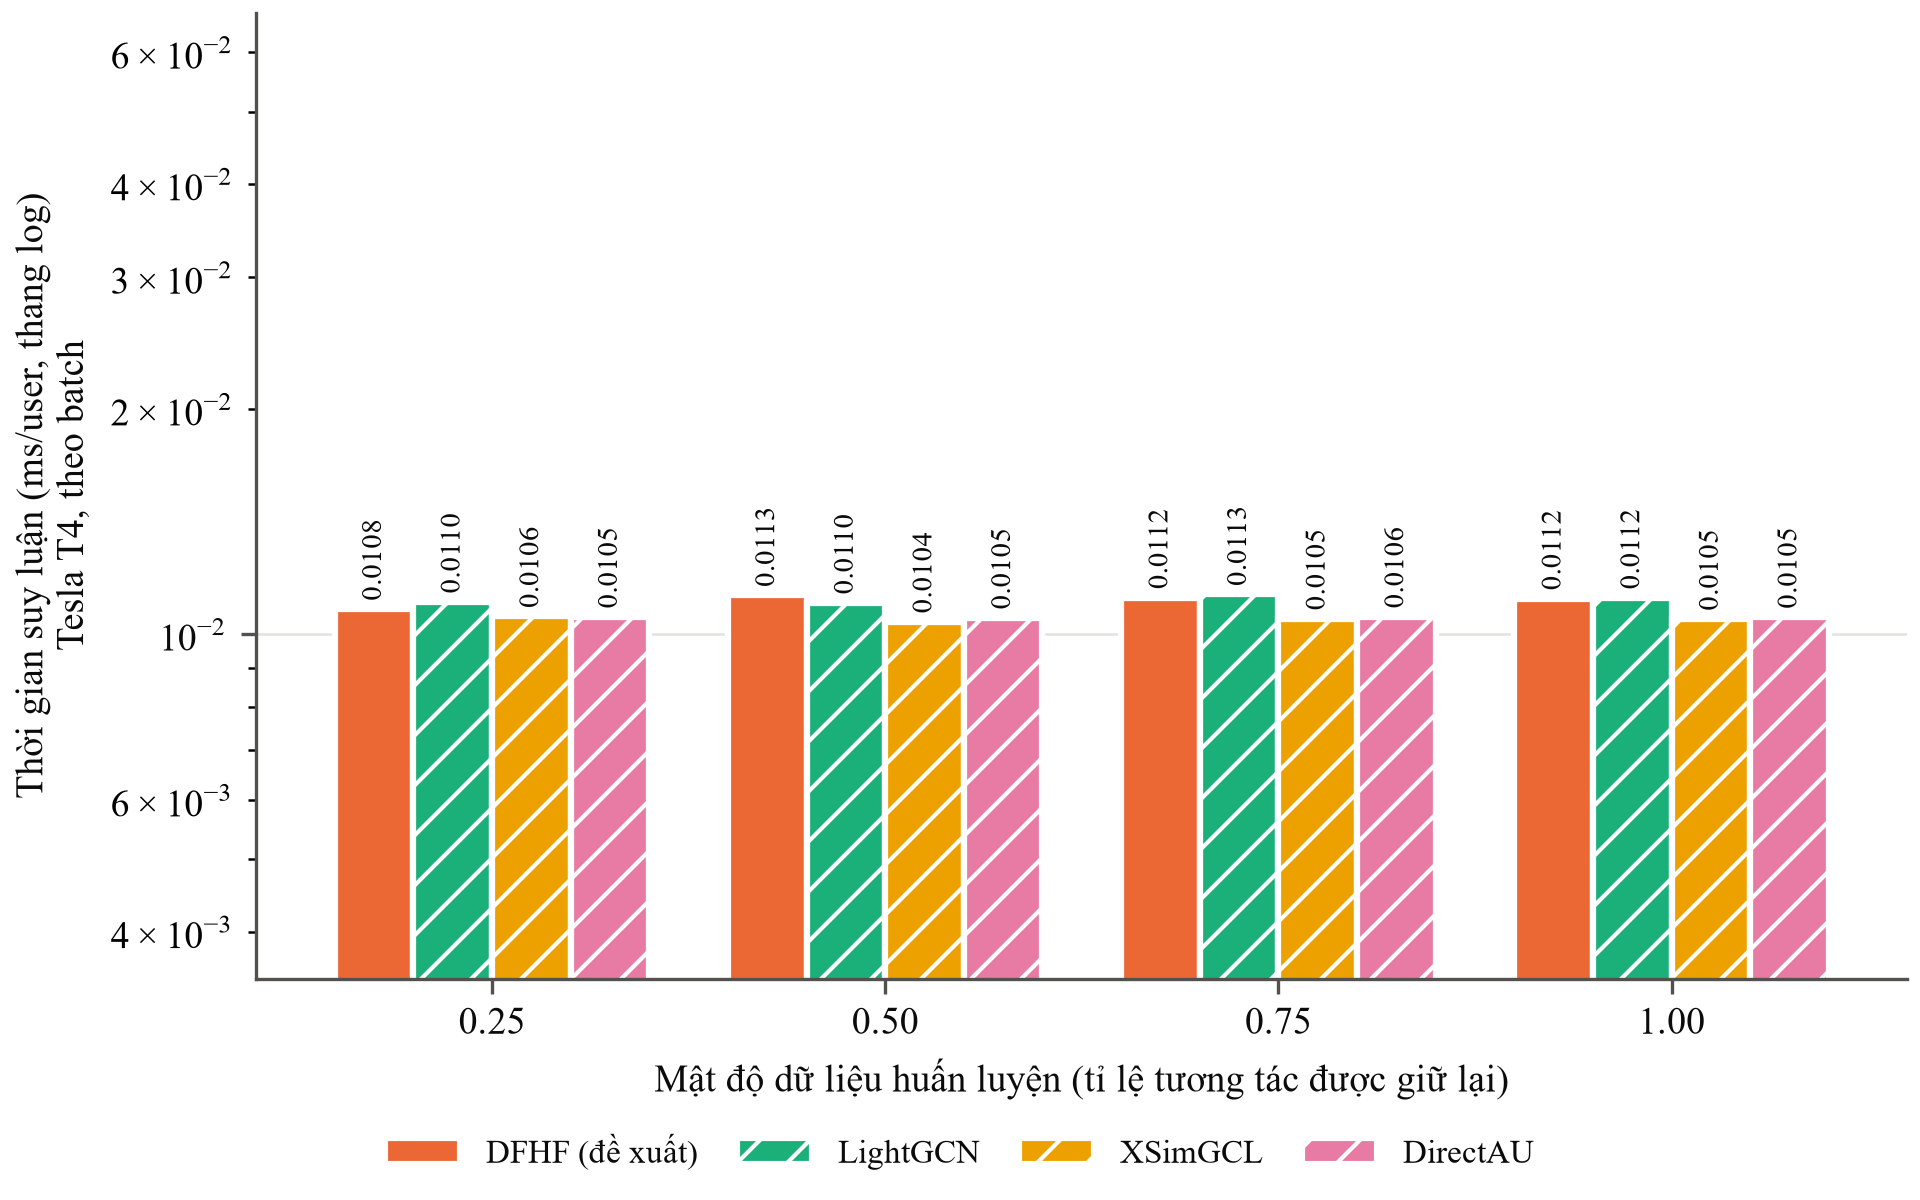
\includegraphics[width=\linewidth]{H7b_trained_inference_latency.png}
\caption[Thời gian suy luận của các mô hình cần huấn luyện]{Thời gian suy luận của các mô hình cần huấn luyện. Thời gian trung bình cho mỗi người dùng khi chấm điểm theo lô trên GPU Tesla T4; trục tung theo thang log, đơn vị ms.}
\label{fig:trained-latency}
\end{figure}

\subsection{Hệ thống demo}
\label{sec:demo}

Dự án xây dựng một ứng dụng Streamlit để minh họa cách các mô hình phục vụ gợi ý. Luồng xử lý gồm bốn bước (\figref{fig:demo-flow}): mô hình được fit hoặc huấn luyện offline và lưu checkpoint; ứng dụng nạp checkpoint vào một bộ xếp hạng dùng chung cho mọi mô hình; bộ xếp hạng chấm điểm các sản phẩm ứng viên; cuối cùng ứng dụng loại các sản phẩm đã có trong lịch sử và hiển thị top-$K$ kèm metadata.

\begin{figure}[htbp]
\centering
\begin{tikzpicture}[node distance=0.5cm, every node/.style={font=\small}]
\node[chthreeblue, text width=2.6cm] (fit) {Fit/huấn luyện offline};
\node[chthreeblue, text width=2.6cm, right=of fit] (ckpt) {Lưu checkpoint};
\node[chthreegreen, text width=2.6cm, right=of ckpt] (rank) {Bộ xếp hạng: chấm điểm ứng viên};
\node[chthreeorange, text width=2.6cm, right=of rank] (ui) {Top-$K$ và metadata trên giao diện};
\draw[chthreeflow] (fit) -- (ckpt);
\draw[chthreeflow] (ckpt) -- (rank);
\draw[chthreeflow] (rank) -- (ui);
\end{tikzpicture}
\caption[Luồng xử lý của hệ thống demo]{Luồng xử lý của hệ thống demo.}
\label{fig:demo-flow}
\end{figure}

Ứng dụng có ba tab. Tab \emph{Gợi ý cho khách} chọn một người dùng có sẵn và hiển thị gợi ý của mô hình được chọn. Tab \emph{Khách mới} cho phép nhập một lịch sử sản phẩm tùy ý; vì cả GRNR lẫn DFHF đều biểu diễn người dùng bằng lịch sử, lịch sử mới được chấm điểm ngay mà không cần huấn luyện lại. Với GRNR, đặc trưng của lịch sử mới được tính giống hệt một hàng train (mỗi sản phẩm có trọng số $1/\sqrt{n}$). Tab \emph{Đánh giá mô hình} hiển thị bảng, kiểm định và biểu đồ, tách riêng nhóm cần huấn luyện và nhóm giải trực tiếp như trong báo cáo.

Riêng GRNR, ứng dụng hiển thị lý do gợi ý: với mỗi sản phẩm được gợi ý $i$, liệt kê các sản phẩm $j$ trong lịch sử có đóng góp $\beta_{ij}/\sqrt{n}$ dương, xếp theo đóng góp giảm dần. Đây là phân rã đại số của điểm GRNR (Mục~\ref{sec:grnr-algorithm}). DFHF không có cơ chế giải thích tương đương.

Hệ thống demo có ba giới hạn. Chưa có đánh giá với người dùng thật, nên không thể kết luận về mức độ hữu ích của gợi ý hay của phần giải thích. Tab \emph{Khách mới} chỉ để minh họa, không phải một benchmark cho người dùng mới. Thời gian phản hồi trong demo cũng không phải số đo của một dịch vụ thực tế.

\subsection{Thảo luận và hạn chế}
\label{sec:discussion}

\textbf{Tóm tắt theo nhóm.} Trong nhóm giải trực tiếp, GRNR có điểm cao nhất ở $d=1$ và $d=0{,}25$, hơn EASE top-128 và GF-CF ở $d=1$, nhưng chưa đủ bằng chứng để nói GRNR tốt hơn EASE đầy đủ ở $d=1$, và thua EASE đầy đủ rõ ràng ở $d=0{,}5$. Ưu điểm rõ nhất của GRNR là chi phí: fit nhanh hơn và lưu trữ nhỏ hơn EASE đầy đủ nhiều lần, với chất lượng gần bằng. Trong nhóm cần huấn luyện, DFHF có điểm cao nhất ở cả bốn mức $d$ với khoảng tin cậy không chứa 0, đổi lại thời gian mỗi epoch dài nhất nhóm và kết quả phụ thuộc mạnh vào việc chọn checkpoint.

\textbf{Độ phổ biến ở mức thưa nhất.} Để đặt các kết quả vào bối cảnh, dự án tính thêm một mốc tham chiếu MostPop: xếp các sản phẩm ứng viên theo số tương tác trong train giữ lại, loại các sản phẩm đã có trong lịch sử. MostPop không thuộc nhóm nào và không phải mô hình đề xuất; nó chỉ cho biết một xếp hạng không cá nhân hóa đạt được bao nhiêu. NDCG@20 của MostPop gần như không đổi theo $d$ (0,0181 ở $d=1$; 0,0177 ở $d=0{,}25$). Ở $d=1$, mọi mô hình trừ GF-CF đều vượt xa mốc này. Ở $d=0{,}25$ thì khác: \emph{không mô hình nào vượt MostPop}. DFHF ngang MostPop ($\Delta=-0{,}00005$, KTC $[-0{,}00029;\,+0{,}00018]$), các mô hình còn lại thấp hơn rõ, kể cả GRNR ($\Delta=-0{,}00973$). Ở $d=0{,}5$, GRNR vẫn thấp hơn MostPop một chút ($\Delta=-0{,}00092$, KTC $[-0{,}00163;\,-0{,}00022]$), còn DFHF cao hơn ($\Delta=+0{,}00459$) (so sánh mang tính mô tả, không hiệu chỉnh đa so sánh). Như vậy, ưu thế của DFHF ở $d=0{,}25$ so với các baseline cùng nhóm phản ánh chủ yếu việc DFHF rơi về thứ tự độ phổ biến cho người dùng chỉ còn một tương tác, trong khi các baseline học vector người dùng từ một tương tác duy nhất và xếp hạng kém hơn cả độ phổ biến. Ưu thế này không nên được hiểu là DFHF học được tín hiệu cá nhân hóa tốt hơn khi dữ liệu rất thưa.

\textbf{Các giải thích cạnh tranh.} Báo cáo chưa có thí nghiệm loại bỏ từng thành phần (ablation), nên mọi giải thích cơ chế dưới đây đều là giả thuyết. (i) Việc DFHF vượt các baseline cùng nhóm ở $d\ge0{,}5$ có thể do bộ lọc khuếch tán và softmax toàn danh mục, nhưng cũng có thể do các baseline chưa được tinh chỉnh tối ưu, chẳng hạn DirectAU chưa hội tụ; muốn phân biệt cần ablation với $F=I$ và tinh chỉnh baseline với cùng ngân sách. (ii) Việc GRNR hơn EASE ở $d=0{,}25$ nhưng thua ở $d=0{,}5$ có thể do giới hạn 128 láng giềng và điều chuẩn theo độ hỗ trợ có lợi khi dữ liệu rất thưa nhưng bó hẹp ở mức trung bình; cũng có thể chỉ là nhiễu của một lần lấy mẫu ở mỗi mức $d$. Lặp lại việc lấy mẫu với nhiều seed sẽ giúp phân biệt. (iii) Việc GRNR gần bằng EASE đầy đủ ở $d=1$ phù hợp với việc cả hai cùng là hồi quy giữa các sản phẩm, nhưng cần thêm bộ dữ liệu để xác nhận.

\textbf{Hạn chế.} Theo thứ tự ảnh hưởng đến kết luận:
\begin{enumerate}
\item \emph{Chọn trên validation.} Checkpoint và cấu hình được chọn trên chính tập validation dùng để báo cáo, nên mọi giá trị tuyệt đối đều lạc quan. Tập test chưa được dùng để xác nhận.
\item \emph{Một seed.} Mỗi mô hình và mỗi mức $d$ chỉ được chạy một lần; khoảng tin cậy không phản ánh biến động giữa các lần huấn luyện hay giữa các lần lấy mẫu train.
\item \emph{Một bộ dữ liệu.} Mọi kết luận chỉ áp dụng cho Amazon Electronics với giao thức đã mô tả.
\item \emph{Tinh chỉnh không cân bằng.} GRNR và DFHF được tinh chỉnh trong quá trình phát triển, còn các baseline dùng cấu hình mặc định hoặc cố định; DirectAU có dấu hiệu chưa hội tụ~\cite{dacrema2019progress,sun2020rigorous}.
\item \emph{Thời gian chỉ chính xác đến ngày.} Có nhiều tương tác validation cùng ngày với tương tác train cuối, nên giao thức không mô phỏng chặt chẽ việc dự đoán tương lai~\cite{ji2023leakage}.
\item \emph{Khác biệt phần cứng.} Các nhóm và một số mô hình chạy trên các máy khác nhau, nên số đo thời gian chỉ mang tính tham khảo.
\item \emph{Bất thường của GF-CF.} Kết quả và thời gian chạy của GF-CF không thay đổi đều theo $d$ và chưa được giải thích; GF-CF chỉ ngang MostPop ở $d=1$.
\end{enumerate}
